
\chapter{人工智能:回顾}

\section{图灵}

在1950年,阿兰·图灵写下了一篇关于人工智能的既有远见又有争议的文章,题目是“计算机器与智能”,发表在《心智》杂志上\note{阿兰·图灵,“计算机器和智能”,《心智》卷LIX,236号,(1950年)。重印于阿·罗·安德森编的《心智与机器》。}。我将会谈到这篇文章,但我想先说说图灵这个人。

\begin{figure}
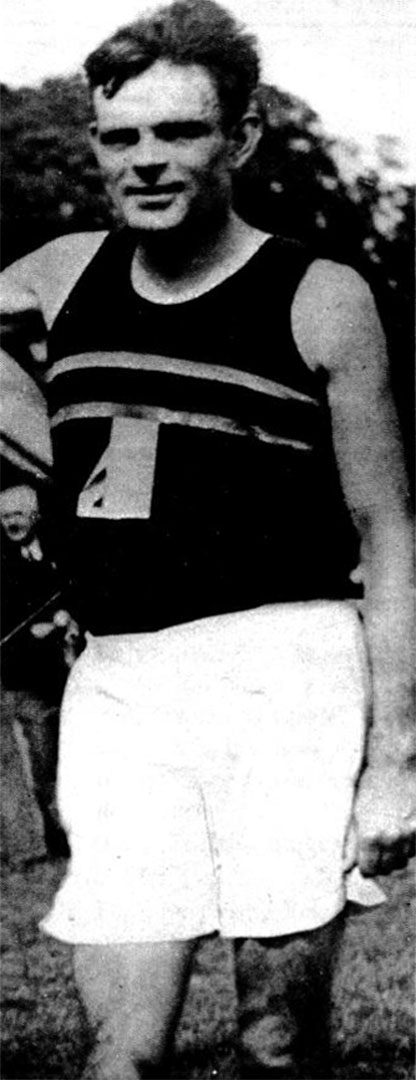
\includegraphics[height=.8\textheight]{img_113.jpg}
\caption[阿兰·图灵。]
  {在赛跑中获胜后的阿兰·图灵(1950年5月)。[摘自萨拉·图灵,《阿兰·图灵》]}
\end{figure}

阿兰·麦瑟森·图灵1921年生于伦敦。当他还是一个孩子的时候,就充满了好奇心和幽默感。由于他的数学天赋,他进了剑桥,在那里他关于机械和数理逻辑的兴趣相得益彰,导致他写出了一篇关于“可计算的数”的著名论文。在这篇论文中,他提出了图灵机理论,而且证明了停机问题的不可解性。这篇论文发表于1937年。在40年代,他的兴趣从计算机理论转向了计算机的实际制造。他在英国的计算机发展史上发挥了重要的作用。人工智能刚刚出现时,面临的是一片攻击与嘲笑,而图灵当时则是它的一名坚定的捍卫者。那时戴维·钱伯农是他最好的朋友之一(此人后来致力于计算机作曲)。他们俩都是国际象棋迷,并发明了“绕屋跑”下棋法:走一步棋后绕房子跑一圈——如果你跑回来时对手还没有走棋,你就有权再走一步。但他们也合作干了件正经事:发明了第一个下棋程序。他们为它起了个名字,叫“图尔钱”。图灵死得很早,才$41$岁——似乎是一次化学事故造成的,也有人说是自杀。他的母亲萨拉·图灵为他写了传记。从她所引用的那些人的话中,人们得到的印象是:图灵不是个循规蹈矩的人,有些不善交际,但又非常诚实正直,因此很容易被他人所伤。他喜爱游戏、下棋、孩子和骑自行车,还是个长跑好手。在剑桥上学时,他买了一把旧小提琴,自己学会了演奏。尽管水平不是很高,他却从中得到了很大乐趣。他有点古怪,对于他感兴趣的事情,他会全力以赴去做,做完便又对另外的什么东西感兴趣了。他所探索的领域之一是生物学的形态发生问题。用他母亲的话说,图灵“特别喜欢《匹克威克外传》”,但“对诗歌——除了莎士比亚的——却丝毫不感兴趣”。阿兰·图灵是计算机科学领域中真正的拓荒者之一。

\section{图灵测验}

图灵的那篇文章是这样开始的:“我准备考虑一个问题:‘机器能思维吗?’”。正像他所指出的,这些词都太复杂了,易于挑起争端,因此我们显然应当寻找一种更好的方式来接近这个问题,即给出一种限定其含义的过程,而非一个定义。他认为这种方式就包含在他所谓的“模拟游戏”之中——今天我们称之为“图灵测验”。图灵是这样介绍的:

\begin{quote}
这种游戏需要三个人来玩:一个男人(A),一个女人(B),以及一个性别不限的询问人(C)。询问人待在一间看不到另外两人的屋子里。游戏的目的是让询问人确定另外两个人谁是男的谁是女的。他只知道这两个人的代号是X和Y,而游戏结束时他要说出“X是A,Y是B”或“X是B,Y是A”。询问人可以这样向A和B提问题:

C:请X告诉我他或她头发的长度。

现在假设X实际是A,那A就必须回答。A在游戏中的目的是设法使C作出错误的判断。这样他的回答就可能是:

“我梳的是短发,最长的一股大约有二十多厘米长”。

为了不让答话的声音给询问人以线索,答案可以写在纸上,要是用打字机就更好了。理想的办法是用电传打字机进行两个屋子之间的通讯。也可以让中间人转述问题和答案。游戏的第三个参加者(B)的目的是帮助询问人。对她来说,最好的策略大概就是提供真实的答案。她可以在答案上加上“我才是那个女的,别听他的话!”或诸如此类的东西。但这于事无补,因为那个男人也可以这样做。

现在我们要问,“如果让一台机器在这场游戏中扮演A的角色,那会发生什么情况呢?”当游戏这样进行时,询问人作出错误判断的可能性是否和参加游戏的是一男一女时一样大?这些问题实际上就是我们原先的那个“机器能思维吗?”的问题。\note{安德森编的图灵文:第5页。}
\end{quote}
在讲清楚他的测验的性质之后,图灵接下去对此作了些评论,这些评论即使在今天看来都很复杂,更不必说在他写作的年代了。开始,他给出了询问人和被询问人之间的一小段假想的对话:\note{安德森编的图灵文:第6页。}
\begin{quote}
\begin{dialogue}[labelwidth=\ccwd,leftmargin=2\ccwd]
\item[问]请以福斯大桥为题写一首十四行诗(这座桥位于苏格兰的福斯河口)。
\item[答]这可把我难倒了。我从来也不会作诗。
\item[问]把$34957$和$70764$相加。
\item[答](停了大约$30$秒然后给出答案)$105621$。
\item[问]你会下国际象棋吗?
\item[答]会。
\item[问]我就剩一个国王在K1,没有别的子了,而你有一个国王在K6,一个车在R1,该你走棋,你怎么走?
\item[答](停了大约$15$秒),车到R8,将!
\end{dialogue}
\end{quote}
可能没有多少读者会注意到,那个算术问题中,不但反应时间异乎寻常地长,而且连答案都是错的!如果回答者是人,就很容易被解释:只不过是个计算错误而已。但如果回答者是台机器,这就可能有许多不同的解释。下面就是某些解释:
\begin{enumerate}
\item 一个偶然的硬件层次上的运行时失误(即不可再现的意外故障);
\item 一个无意中出现的硬件(或程序)故障,它可能造成算术运算中的错误(可再现的);
\item 一个由该机器的程序员(或制造者)有意插入的花招,它可能不时造成算术运算中的错误,以此来迷惑询问人;
\item 一个不可预测的旁效现象:程序由于长期进行艰苦的抽象思维,偶然出了点小错,下次就不会再错了;
\item 一个由机器自己想出来的玩笑,故意戏弄询问人。
\end{enumerate}
要搞清图灵在这里到底是什么意思,就涉及到和人工智能有关的几乎全部的重大哲学问题。

图灵接下去指出:
\begin{quote}
这个新问题的优点在于把人的物理能力和心智能力明确地区分开了……我们不想因为一台机器不能参加选美大赛而责备它,就像我们不会因为一个人没有飞机速度快而责备他一样。\note{安德森编的图灵文:第6页。}
\end{quote}
读这篇文章时的一大乐事就是看图灵怎样展开他的每条思路。通常他总是在某个阶段摆出一种似乎是矛盾的东西,然后通过修正他的概念,再在分析的更深层次上解决。由于这种对问题入木三分的剖析,在计算机有了长足的发展,人工智能也进行了深入的工作的近三十年之后,这篇文章仍放射着耀眼的光辉。在下面的引文中你可以看到思想的这种往复工作方式:
\begin{quote}
也许有人会指责说这种游戏的设计对机器太不利了。如果那个人想装成机器,很显然他会把事情搞糟。仅在做算术题时又慢又不准确这一点上就足以让他漏馅了。难道说机器就不能完成某种应当被描述成思维、但又与人所具有的完全不同的东西吗?这种反对意见是很有力的,但至少我们可以说,如果能构造出一台能令人满意地玩这种模拟游戏的机器来,那我们就不必为这种意见所烦扰。

有人也许认为机器在玩这种“模拟游戏”时最好的策略可能并不是模拟人的行为。也许会是这样的,但我认为即使如此似乎也不会造成很大的影响。无论如何这里并不打算探讨博弈论,而且我们假定最好的策略就是设法提供那种人会很自然地给出的答案。\note{安德森编的图灵文:第6页。}
\end{quote}
当这种测验被提出并讨论之后,图灵写到:
\begin{quote}
至于原来那个问题——“机器能思维吗?”,我相信它没什么意义,不值得讨论。不过,我相信到本世纪末,词的用法和广大受过教育的人的看法会发生很大的改变,因此那时将可以谈论机器思维而不怕再造成矛盾了。\note{安德森编的图灵文:第13--14页。}
\end{quote}

\section{图灵所预料的反对意见}

由于图灵知道这种观点无疑会遇到暴风雨般的反对,他接着就简洁而又带有幽默感地剖析了一系列对“机器能够思维”这种想法的反对意见。我在下面给出他列出的九类反对意见,并采用他自己对它们的描述方式。\note{安德森编的图灵文:第14--24页。}遗憾的是,由于篇幅所限,这里不能复述他所给出的幽默而又机智的答复了。你也许会乐于自己思考一下这些反对意见,并给出你自己的答复。
\begin{enumerate}
\item 来自神学的反对意见:思维是人的不朽的灵魂所具有的功能。上帝把不朽的灵魂赐给了每个男人和女人,但没有赐给任给其它动物或机器。因此动物和机器都是不能思维的。
\item 鸵鸟式的反对意见:机器思维的后果将是非常可怕的。让我们希望并且相信它们不能做到吧。
\item 数学化的反对意见\lnote{(这基本上就是卢卡斯的论点)}。
\item 基于意识的论点:“除非一台机器能出于自身的思想和情感——而不是据符号的任意组合——写出一首十四行诗或一首协奏曲,否则我们不能同意说机器等于大脑——这就是说它不但要能写出来,还要能知道它已经写出来了。没有什么机器能够真正产生下列感受(而不仅仅是发出人为设置的信号——那是简单的发明):在它成功时感到愉快,在它的部件损伤时感到痛苦,听到奉承话就觉得舒服,犯了错误就觉得悲伤,碰到异性会被吸引,得不到它想要的东西就会愤怒或失望。”\lnote{(这是援引某位杰弗逊教授的话。)}
\end{enumerate}
图灵非常希望能对这种严厉的批评作出圆满的答复。因此,他为他的答案提供了不小的篇幅,而且在其中他又提供了一段假想的对话:\note{安德森编的图灵文:第17页。}
\begin{quote}
\begin{dialogue}[labelwidth=3\ccwd,leftmargin=4\ccwd]
\item[询问人]你的十四行诗中的第一行是:“我怎能把你比作夏天”,为什么不是“春天”呢?那样不是更好吗?
\item[被问者]那样就不符合格律了。
\item[询问人]那么“冬天”怎么样?这符合格律。
\item[被问者]对,但谁也不想被比作冬天。
\item[询问人]提到匹克威克先生,是否会令你想到圣诞节?
\item[被问者]可以这么说吧。
\item[询问人]因为圣诞节是在冬天,所以我想你如果把匹克威克先生比作冬天,他是不会计较的。
\item[被问者]我觉得你不是在严肃地讨论问题。提到冬天,我们总是指冬天的一个一般的日子,而不是指像圣诞节这样特殊的日子。
\end{dialogue}
\end{quote}
在这段对话之后,图灵问道:“如果一台能写十四行诗的机器在口试时能这样回答问题,那杰弗逊教授还有什么话说呢?”其它的反对意见还有:
\begin{enumerate}[resume]
\item 基于各种缺陷的论点:“就算你能造一台机器做你所提到过的那些事,你也绝不可能造出一台能做到X的机器。”有许多与此相关的X被提了出来。我在下面提供其中一部分:善良、机智、优美、友好、有创造性、有幽默感、区别是非、犯错误、坠入情网、爱吃草莓和奶油、使人动心、从经验中学习、用词得当、成为自己思考的对象、像人那样行为多变、做某些真正新的事情。
\item 洛芙莱丝命妇的反对意见:关于巴比奇的分析机,最详尽的信息来自洛芙莱丝命妇所写的一本传记。她在其中写到:“分析机并不自称能\textsf{\bfseries 创造}任何东西。它能做\textsf{\bfseries 任何我们知道怎样命令它去做的事}”\lnote{(黑体是她用的)}。
\item 基于神经系统连续性的论点:神经系统肯定不是一台离散状态的机器。一个撞击神经系统的神经脉冲的强度这样的信息若是有一点误差,都可能使输出脉冲的大小产生很大差别。因此可以争辩说,由于这个原因,我们不能指望用一个离散状态系统来模拟神经系统的行为。
\item 基于行为非形式化的论点:这种观点大概是这样的:“如果每个人都有一个确定的指导规则集来控制他的生活,那他也就无异于机器了。但并不存在这种规则,因此人也就不可能是机器。”
\item 基于超感官知觉的论点:假设我们要进行那种模拟游戏,而两个被问者一个是能接受心灵感应的人,另一个是数字计算机。询问人可以问这样的问题:“我右手里这张扑克牌是什么花色的?”那个人利用心灵感应或特异功能,在$400$次询问中能说对$130$次。而那台机器只能随机地猜测,也许只能说对$104$次,这样,询问人就能作出正确的判断了。
\end{enumerate}

正如你所能看到的那样,许多反对意见彼此重叠、互相联系。我已经在本书中设法对其中的大多数作出了这样或那样的回答,但一般都不如图灵的那么简洁。

我觉得第9种反对意见是值得注意的。我曾见到图灵这篇文章被重印在某本书里,但第9种反对意见被略去了——我觉得这同样是值得注意的。我自己的观点——和图灵的相反——是认为超感官知觉并不存在。图灵也不想承认真的有超感官知觉,不过后来还是被迫承认了,原因是他那种杰出科学家的诚实精神要求他接受他认为是强有力地支持了超感官知觉的统计证据。我不这样看,尽管我把这个问题当成一个极其复杂而迷人的问题。

\section{“帕里遇上了医生”}

在本章前面的对话中,你已经看到了计算机程序和人交谈时的真实情况。还有许多“交谈”能力比施德鲁差的程序。其中有两个很著名,一个是约瑟夫·魏增鲍姆设计的“医生”,另一个是肯尼思·科尔比设计的“帕里”。前者是要模拟一个使用“启发式疗法”的精神病医生——也就是那种只靠问问题来治病的心理医生,而后者是要模拟一个妄想狂患者的信念结构。人们通过计算机网为这两个程序安排了一次有趣的正面较量,下面就是谈话记录中的一小段:\note{文顿·瑟夫[Vinton Cerf],“帕里遇见了医生”?第63页。}
\begin{quote}
\begin{dialogue}[labelwidth=2\ccwd,leftmargin=3\ccwd]
\item[帕里]我不理解你的动机。
\item[医生]你为什么不理解我的动机呢?
\item[帕里]我难道不应该吗?
\item[医生]你为什么现在这样说?
\item[帕里]事实就是如此。
\item[医生]假设事实并不是如此。
\item[帕里]然后呢?
\item[医生]我不知道我是否完全理解你了。
\item[帕里]你总是唠叨同一个问题。
\item[医生]这种相似性对你有什么启发?
\item[帕里]我不太明白你的意思。
\item[医生]你希望你太明白我的意思吗?
\item[帕里]你现在该对我的感情表现出兴趣了。
\item[医生]哦?我对你的感情表现出兴趣了吗?
\end{dialogue}
\end{quote}
当然,这些程序是被设计来和人谈话的,因此它们在这里互相对话时表现得很糟糕。它们大多是依赖于对输入的性质进行巧妙的猜测(它们对输入的分析十分肤浅),然后在大量事先准备好的回答中仔细地选出一些,再把它们吐出来。这些答案可能仅仅是部分地预先设计好的。例如,可能是一块模板,其中有些空白可供填写。其实是假定和它们交谈的人会从它们所说的话中读出比实际要多的意义来。事实上,按照魏增鲍姆在其著作《计算机能力和人类理性》中所说的那样,情况也的确是如此。他写道:

\begin{quote}
“伊莉莎”\lnote{(即生成“医生”的那个程序)}在与它交谈的许多人心中造成了很强烈的错觉,使他们感到它已经理解了他们所说的话。……他们常常要求与该系统私下交谈。而且在谈了一段时间之后,尽管我作出了解释,他们仍会坚持说机器真的理解了他们。\note{约瑟夫·魏增鲍姆,《计算机能力与人类理性》,第189页。}
\end{quote}

对于上面谈到的这种情况,你可能会感到难以置信。的确难以置信,但这是真的。魏增鲍姆对此提供了一种解释:

\begin{quote}
大多数人对计算机一无所知。因此,除非他们抱有极强的怀疑心理(就像我们在看魔术表演时那样),否则他们如果想解释计算机的那些智能行为,就只能采用他们所能采用的唯一的类比,即类比于他们自己的思维能力模型。这样一来,他们那些过火的想法也就不足为怪了。比如说,的确无法设想一个人能够模拟“伊莉莎”的行为,对他来说“伊莉莎”的语言能力构成了他的极限。\note{魏增鲍姆书,第9--10页。}
\end{quote}
这就相当于承认,这种程序基本上是虚张声势和连蒙带唬的一种巧妙的混合,是利用了人们的轻信心理。

根据这种稀奇古怪的“伊莉莎效应”,有些人提出应当对图灵测验进行修正,因为显然用极简单的花招就可以使人上当受骗。还有人提议询问人应当由得过诺贝尔奖的科学家来担任。更可取的办法可能是把图灵测验反过来,要求询问者也应当由一台计算机充当。或者说设立两个询问者——一个人和一台计算机——和一个被问者,这两个询问者要设法说出这个被问者是人还是计算机。

更严格来说,我个人认为图灵测验的原始形式是很合理的。至于对那些魏增鲍姆宣称被“伊莉莎”所骗的人们来说,问题在于没有提醒他们保持怀疑精神,用全部智慧来设法确定和他们笔谈的那个“人”是否真的是人。我认为图灵对这个问题的见解是正确的,因此图灵测验会本质上保持不变地存在下去。

\section{人工智能简史}

我希望能用下面几页的篇幅,以一种可能是非正统的观点,来讲述某些旨在阐明“智能背后的算法”的努力。我们已经遇到了许多错误和挫折,今后还会是这样。但不管怎么说,我们还是学到了许多东西,而且这的确是一个激动人心的时期。

甚至从帕斯卡和莱布尼茨开始,人们就梦想着用机器来完成智能性的任务了。在十九世纪,布尔和德·摩根发明了“思维定律”——本质上就是命题演算——因此就迈出了通往人工智能软件的第一步。查尔斯·巴比奇设计了第一台“计算机械”——现代计算机硬件的前身,也就是人工智能硬件的前身。我们可以把人工智能出现的时刻定义成机械装置完成了某些以前只能用人脑完成的任务之时。现在很难回过头去想象,那些人初次看到齿轮能完成大数的加法和乘法时会有何感想。或许他们在看见“思想”从物理的硬件中涌流而出时,体验到了一种敬畏之感。无论怎样说,我们确实知道,在近一个世纪之后,当第一台电子计算机构成的时候,其设计者们是体验到了在面对另一种“思维生物”时的一种敬畏、神秘之感。在那种情况下到底在多大程度上发生了真正的思维,这是许多困惑的根源所在。甚至在几十年后的今天,这个问题仍是刺激与苦恼的一个丰富的源泉。

有趣的是,今天实际上已经没有人再有敬畏感了——尽管和当时那些令人后脊梁骨上冒凉气的东西相比,现在计算机所完成的工作已经复杂得令人不可思议了。“大电脑”这个一度使人激动不已的名词现在只不过是一个过时的陈词滥调,成了旧时代的一个可笑的遗迹。我们这样快就对它感到厌倦了,这多少有点令人悲哀。

有一个与人工智能的进展相关的“\emph{定理}”:一旦某些心智功能被程序化了,人们很快就不再把它看作“真正的思维”的一种本质成分。智能所固有的核心永远是存在于那些尚未程序化的东西之中。这个“\emph{定理}”是拉里·泰斯勒首先向我提出的,因此我称它“\emph{泰斯勒定理}”:“人工智能是尚未做到的东西”。

下面我来对人工智能作一个有选择的概述,以展示若干个集中了研究者努力的领域,其中每个领域似乎都以其自身的方式需要智慧的精华。对其中的某些领域,我又根据所使用的方法或所特别关注的问题作出了更细致的划分。

\begin{itemize}
\item 机器翻译
  \begin{itemize}
  \item 直接的(词序重新排列过的查字典过程)
  \item 间接的(通过某种作中介的内部语言)
  \end{itemize}
\item 博弈
  \begin{itemize}
  \item 国际象棋
    \begin{itemize}
    \item 盲目的超前搜索
    \item 带修剪机制的启发式超前搜索
    \item 无超前搜索
    \end{itemize}
  \item 跳棋
  \item 围棋
  \item 五子棋
  \item 桥牌(叫牌和打牌)
  \item 扑克
  \item 三子棋的各种变形
  \item 等等
  \end{itemize}
\item 数学各分支中的定理证明
  \begin{itemize}
  \item 符号逻辑
    \begin{itemize}
    \item “归结法”定理证明
    \end{itemize}
  \item 初等几何
  \end{itemize}
\item 数学表达式的符号处理
  \begin{itemize}
  \item 符号积分
  \item 代数式化简
  \item 无穷级数求和
  \end{itemize}
\item 视觉
  \begin{itemize}
  \item 印刷品:
    \begin{itemize}
    \item 识别取自某小集合中的单个手写字符(如数字)
    \item 阅读各种字体的西文文字材料
    \item 阅读手写的西文段落
    \item 阅读印刷体的中文或日文
    \item 阅读手写体的中文或日文
    \end{itemize}
  \item 图像:
    \begin{itemize}
    \item 在照片上寻找事先说明的物体
    \item 把一幅图像分解成独立的物体
    \item 在一幅图像中辨识出独立的物体
    \item 根据人提供的简图识别物体
    \item 识别人的面容
    \end{itemize}
  \end{itemize}
\item 听觉
  \begin{itemize}
  \item 在有限的词汇范围内理解口头表达的词(如十个数字的名称)
  \item 固定的领域中理解连续的话语
    \begin{itemize}
    \item 找到音素间的界限
    \item 辨识音素
    \item 找到词素间的界限
    \item 辨识词素
    \item 整合出完整的词和句子
    \end{itemize}
  \end{itemize}
\item 自然语言理解
  \begin{itemize}
  \item 在特定领域中回答问题
  \item 复杂句的语法分析
  \item 对文字材料进行分段
  \item 使用关于现实世界的知识以理解一段话
  \item 解决有歧义的指称关系
  \end{itemize}
\item 自然语言生成
  \begin{itemize}
  \item 抽象的诗(如俳句)
  \item 随机的句子、段落成更长的文字片段
  \item 从内部知识表示中产生输出
  \end{itemize}
\item 构造有独创性的思想或艺术作品
  \begin{itemize}
  \item 写诗(如俳句)
  \item 写小说
  \item 计算机绘画
  \item 音乐创作
    \begin{itemize}
    \item 无调性的
    \item 有调性的
    \end{itemize}
  \end{itemize}
\item 类比思维
  \begin{itemize}
  \item 几何形状(“智力测验”)
  \item 根据一个数学领域中的证明构造另一个相关领域中的证明
  \end{itemize}
\item 学习
  \begin{itemize}
  \item 参数调整
  \item 概念形成
  \end{itemize}
\end{itemize}

\section{机器翻译}

在我下面要进行的讨论中,我将有所选择,略去上面列出的一些课题。不过,把它们列出来也是必要的,否则这份清单就不准确了。前面的几个课题是按历史次序排列的,每一个课题都没有达到预期的目的。例如,在机器翻译中所遇到的障碍使许多人大吃一惊。他们原以为这大概是个简单明确的任务,要做得尽善尽美的确很难,但基本上实现应该是很容易的。然而实践证明,翻译远不只是查字典和把词重新排列所能完成的。难点也不仅在于缺乏关于习惯用语的知识。事实上,翻译涉及到要为所讨论的领域建立一个心智模型,然后去处理那个模型中的符号。一个程序如果在读入文章段落时不使用一个领域模型,那它不久就会在遇到意义不清或多重意义时毫无希望地陷入困境之中。甚至一个人——他和计算机相比占有很大的优势,因为他对这个世界具有深入的理解——给他一段用他不懂的语言写成的文章和一本字典的时候,也会发现他几乎不可能把这段文字翻译成他自己的语言。因此——这在回顾时就不足为奇了——人工智能的第一个难题立即就涉及到了人工智能的核心问题。

\section{计算机弈棋}

计算机下国际象棋也被证明比开始时的直觉估计所设想的要困难得多。在这里,实践再次说明,人在心里表示一个棋局的方式,要远远复杂于仅仅知道哪个棋子在哪个位置上,以及下棋的规则。这涉及到感知若干相关的棋子所形成的结构,以及“启发式”的知识(或者说是估计),因此与高层组块有关。虽然不像正式规则那样严格,但启发式规则为了解棋盘上进行的事件提供了捷径,而正式规则是不能提供这种知识的。人们对这一点在一开始就有所认识,但只是过低地估计了对棋局的这种直观的、组块化的理解在人的棋艺中所起的巨大作用。当时的预想是,一个程序只要具有某些基本的启发式规则,再加上计算机在对局时进行盲目的超前搜索时的速度和精度,通过对每种可能的步骤进行分析,就能轻而易举地击败第一流的人类棋手——这个预想甚至在许多人紧张地工作了二十五年之后的今天,仍然远远没有成为现实。

时至今日,人们在从不同的角度处理下棋问题,其中最新颖的想法之一就是认为超前搜索是劳而无功的。反之,我们只需看看当前的局势是怎样的,并使用某些启发式规则生成一个计划,然后寻找一个能推进这个特定计划的棋步。当然,下棋计划的形成规则中必须要包括一些启发式知识,它们在某种意义下是超前搜索的“压缩”形式。这就是说,在许多盘棋中的超前搜索经验的等价物被“凝固”成另一种形式,而这种形式表面上并不需要超前搜索。在某种意义下这是个文字游戏。但如果这种“压缩的”知识在提供回答时比实际的超前搜索更有效——即使它偶尔会误入歧途也罢——那我们就已经有所收获了。像这样把知识蒸馏成更有效的形式,正是智能的长处所在,因此在下棋时更少地进行超前搜索,可能是进行研究时的一条行之有效的路径。尤其吸引人的想法是设计这样一个程序,它自己能把从超前搜索中得到的知识变换成“压缩的”规则——但这是个艰巨的任务。

\section{塞缪尔的跳棋程序}

事实上,在阿瑟·塞缪尔所设计的令人赞赏的跳棋程序中,已经采用了这样一种方法。塞缪尔所用的技巧是同时使用“动态”(超前搜索)和“静态”(非超前搜索)两种方式来评价任何给定的棋局。

静态方法采用一个由若干适用于任意棋局的特征量所构成的简单函数,这样就可以立即实际计算出来。而动态估值方法需要构造一棵“树”,其中表示了所有后面可能出现的棋步、对它们的反应、对这些反应的反应,如此等等(如\fig{38}所示)。在静态估值函数中有一些可以改变的参数,对它们进行改变的结果就会提供一组静态估值函数的可能的不同形式。塞缪尔的策略是以一种渐进的方式为这些参数选择越来越好的值。

该过程是这样完成的:每当程序要对一个棋局进行估值时,它既静态进行也动态进行。通过超前搜索所得到的答案——让我们称它D——被用来确定下一步要走的棋。而静态估值的结果S被用于一种更巧妙的目的:在每一步中,都对那些可变参数进行轻微调整,以使得S尽可能地接近D。这样做的结果是使通过对树的动态搜索所得到的知识被部分编码于静态估值函数的参数值里了。简而言之,基本想法就是把复杂的动态估值方法“压缩”到简单得多也有效得多的静态估值函数中来。

这里有一种良好的递归效应。这是因为对任意一个棋局的动态估值都需要进行有限步数的超前搜索——比如说七步。这样一来,走了七步之后所遇到的那些棋局本身也需要以某种方式进行估值。但当程序对这些局势进行估值时,它显然不能再超前搜索七步了,否则它将不得不超前搜索十四步,然后是二十一步,如此等等——这是一种无穷回归。因此,它在超前搜索七步后就必须依赖于静态估值了。这样,按照塞缪尔的办法,一种复杂的反馈就出现了。只要程序不断地设法把超前搜索估值“压缩”到一个较简单的静态方法中,这种方法转过来就会在动态的超前搜索估值过程中发挥关键性的作用。于是两种方法就密切地联系起来了,而且每种方法都以递归的方式从另一种方法的改进中受益。

塞缪尔的跳棋程序棋艺高强,基本达到了世界上最好的棋手的水平。如果是这样的话,那为什么不把同一技术应用于国际象棋呢?为了研究计算机下国际象棋的可行性,在1961年召集了一个国际性的委员会,其中包括荷兰的国际象棋特级大师兼数学家麦克斯·尤伟,委员会所得到的结论是前景暗淡:塞缪尔的技术如想应用于国际象棋,则难度大约是应用于跳棋的一百万倍,这似乎等于宣布此路不通。

这个跳棋程序所拥有的高超棋艺不能被解释成“已经达到了智能”,但对它也不能估计过低。在这个程序中结合了若干方面的知识,包括跳棋是什么、如何思考跳棋问题、以及怎样编程序。有些人可能会觉得它所表现出来的实际上是塞缪尔本人的下棋本领。但这是错的,原因至少有两个。其一是棋艺高超的棋手在选择棋步时所依赖的心智过程,往往连他们本人也无法全部理解——他们在使用自己的直觉。现在还没人知道怎样才能揭示自己的所有直觉。我们在内省过程所能采用的最好方法是使用“感受”或“元直觉”——这是一种关于直觉的直觉——作为向导,并且设法描述我们认为我们自己的直觉是什么样子的。但这只不过是为直觉方法的真实的复杂性提供了一种粗略的近似而已。因此实际上塞缪尔肯定无法把他个人的下棋方法映射到他的程序中去。说塞缪尔的程序的棋术不应与塞缪尔本人的棋术相混淆的另一个理由是:塞缪尔的跳棋还不如他的程序下得好——它能赢他。这一点也不会造成悖论——就好像事实上如果给一台计算机编上计算$\uppi$值的程序,那么它一定会比给它编这个程序的人算得快。

\section{程序何时才有独创性?}

这个程序超过其设计者的论题联系着人工智能中的“创造性”问题。如果一个人工智能程序想出了一个主意、或一个下棋时的策略,而这是其设计者所从未想到的——那该归功于谁呢?关于这一点,已经出现了各种有趣的实例,其中有一些是微不足道的,但也有一些涉及到很深的层次。最著名的例子之一是一个为初等欧几里得几何中的定理寻找证明的程序。这个程序的最初构思来自马尔文·明斯基,实际设计者是IBM公司的赫伯特·吉伦特。有一天,这个程序为一个基本几何定理找到了一个精妙绝伦的证明——这个定理就是所谓“ponsasinorum”,即“驴桥”。它得了这么个诨名,是因为头脑简单的人很难通过它。

\begin{lrbox}{\TEMPBOX}%
\begin{tikzpicture}
  [every node/.style={draw=none,inner sep=0pt,outer sep=.3333em}]
\draw    (0,0)   node[left]  {$P$}
      -- (2,0)   node[right] {$P'$}
      -- (1,2.5) node[above] {$A$}
      -- cycle;
\end{tikzpicture}
\end{lrbox}

\begin{figure}
%\includegraphics{img_114.png}
\fcapside[\FBwidth]{\usebox\TEMPBOX}{%
\caption[“驴桥”的证明。]
  {“驴桥”的证明(由帕普斯[约公元300年]和吉伦特的程序[约公元1960年]所发现)。问题:证明等腰三角形二底角相等。解:由于该三角形是等腰的,故$AP$和$AP'$等长,因此三角形$PAP'$和三角形$P'AP$是全等的(边、边、边)。这就说是对应角是相等的。具体来说,两个底角是相等的。}}
\end{figure}

这个定理说:一个等腰三角形的两个底角是相等的。它的标准证明要求作底边的高线,把三角形分成对称的两半。这个程序发现的高明方法(见\fig{114})不需要辅助线。这种方法是把这个三角形和它的镜像看成两个不同的三角形。然后,证明它们是全等的,并据此指出二底角在这一全等关系中彼此对应,这就证明了它们相等。

这个绝妙的证明使程序的设计者和其他人大为兴奋,有些人在它的行为中看到了创造才能的证据。实际上,在公元300年几何学家帕普斯已经发现了这个证明,但这一事实并没有使这项成就黯然失色。不管怎么说,下述问题依然存在,即“功劳该归于谁?”。这能算是智能行为吗?还是说这个证明本来是深藏在人(吉伦特)的心里,计算机只不过是使它浮到表面上来了?后面这个问题差不多打中了要害。我们可以把它反过来:证明是本来深藏在程序之中,还是接近程序的表面?这也就是要问,要使多大劲才能看清程序为什么要做它所做的事?程序的发现是否能归因于其中某个简单的机制,或机制的简单组合?也许,这里存在着一种复杂的相互作用,即使我们听到了对它的解释,也不会减少我们对它的出现所产生的敬畏之感?

我们似乎完全可以这样说:如果我们能把程序的行为归因于其中某些容易被追踪的操作,那在某种意义上,程序所做的只不过是揭示出那些在本质上是埋藏在——虽然并不很深——程序设计者头脑中的想法。相反地,如果对程序的追踪无助于说明为什么这个特定的发现得以产生,那我们也许应当开始把程序的“头脑”与其设计者的头脑加以区别了。程序的构造应归功于人,但不能说在他的头脑里已经有了程序所产生的那些想法。在这种情况下,人可以被说成是“元作者”——即作者的作者,而程序是(普通的)作者。

在吉伦特及其几何机器这种特定的情况下,尽管吉伦特可能并没有重新发现帕珀斯的证明,产生这一证明的机制离程序表面还是太近了。这使得我们难于毫不犹豫地认为该程序本身就有资格被称为一个几何学家。如果这个程序一而再、再而三地提出机智得令人吃惊的新证明,而且其中的每一个看起来都是基于天才的思想火花,而不是基于某种标准的方法,那时我们会坦然地把这个程序称为一个几何学家——但这种情况尚未出现。

\section{计算机音乐是谁创作的?}

作者与元作者之间的区别在计算机作曲的情况下表现得尤为突出。在作曲过程中,一个程序看上去拥有不同层次上的自主权。在以贝尔实验室的麦克斯·马修斯为“元作者”的一段曲子中就表现了其中的一种。他把两首进行曲的乐谱送入了计算机,一首是《约翰尼回家乡》,另一首是《英国掷弹兵》,并要求计算机生成一首新的乐曲——它开始时是“约翰尼”,但要慢慢变成“掷弹兵”,当乐曲演奏到一半的时候,“约翰尼”完全消失了,我们只能听到“掷弹兵”……然后这一过程又反了过来,当乐曲结束时,又和开始时一样,只剩下“约翰尼”了。用马修斯的话说,这是

\begin{quote}
……一个令人厌恶的音乐实验,但也并非毫无趣味,尤其是在节奏的转换上。“掷弹兵”本来是$2/4$拍子、F大调,而“约翰尼”本来是$6/8$拍子、E小调。从$2/4$拍子变成$6/8$拍子可以很清楚地被鉴别出来,虽然音乐家演奏起来很困难。从F大调转到E小调,这就要求在音阶中改变两个音符,结果听起来很刺耳,因而一个更小一点的转调无疑会是个更好的选择。\note{马修斯与罗斯勒[M. Mathews; L. Rosler]:“用于计算机发声的图形语言”,载封·福尔斯特和鲍尚[H. von Foerster; J. W. Beauchamp]所编《计算机作曲》[\bn{Music by Computer}],第96页。}
\end{quote}

这样生成的曲子听起来有点奇异之感,虽然有些地方是浮华而混乱的。

\begin{quote}
是计算机在作曲吗?最好还是不要提这个问题,但对它也不能完全置之不理。要提供一个答案是很难的。所用的算法是确定的、简单的,也不难理解。其中并没有涉及复杂的或难以理解的计算,没有使用“学习”程序,没有出现随机过程,机器是以一种完全机械化的、简单明确的方式在运行。但是,其结果是一个并没有被作曲家完全计划好其细节的声音序列,尽管这一段的总体结构是被完全、精确地说明了的。这样,作曲家就常常吃惊地、而且是又惊又喜地看到了他的想法的实现细节。计算机只是在这种意义下作曲。我们称这一过程为算法化的作曲,但我们马上要再一次强调这些算法是能一目了然的。\note{福尔斯特和鲍尚书,第106页。}
\end{quote}

这就是马修斯对那个他认为最好“废问”的问题的答复。但尽管他拒不承认,许多人还是发现简单地把这段曲子说成是“计算机作的”更方便。我觉得这种说法完全歪曲了实际情况。这个程序中没有任何结构类似于人脑中的“符号”,在任何意义下也不能说它在“思考”它所做的事。把这样一段音乐的创作归功于计算机,就像把本书的创作归功于产生它的计算机编辑照排系统一样。

这就引出了一个问题,这个问题不在人工智能领域中,但离得也并不远。这就是:如果你在一段文字中看到“我”这个字,你认为它指的是什么呢?举例来说,如果你在一辆脏汽车上发现“洗我”这样两个字,那这个“我”是指谁呢?也许这是某个可怜的孩子的呼声,他非常想洗个澡,所以就随便在一个地方乱画出了这两个字?也许是这辆车需要洗刷?也许是这句话想洗一次淋浴?也许,还有可能是要求把我们语言中那些乌七八糟的东西清洗干净?你可以把这个游戏继续做下去。在这里,这两个字是一个玩笑,是设想你在某个层次上会假装相信是这辆汽车自己写了这两个字,要求把它洗刷一下;而在另一个层次上,你又能清楚地看出这是一个孩子的恶作剧,他看着别人产生了误解,觉得很好玩。事实上,这种游戏是基于在不适当的层次上看“我”这个字的。

这种歧义现象在这本书里也已经出现过了,先是在《对位藏头诗》中,后来是在对哥德尔串G(及其相关物)的讨论之中。对不可播放的唱片的说明是:“我不能在唱机X上播放”,对不可证明的判断的说明是:“我不能在形式系统X中被证明”。让我们以后一句话为例。在任何别的场合,当你碰到一句包含有代词“我”的话语,你是否还可能自然地认为它不是指说这句话的人,而是指这句话本身?我猜这种可能性很小。“我”这个词如果出现在莎士比亚的一首十四行诗里,那它指的绝不是印在纸上的这十四行诗句,而是指幕后那个有血有肉的人,这个人是不在场的。

我们通常把一句话中的“我”追溯到多远呢?其答案在我看来,是我们要找到一个有感知力的主体,认为他(它)就是说这句话的人。但什么是一个有感知力的主体呢?是指我们可以方便地拟人化的东西。在魏增鲍姆的“医生”程序中,是否存在一个人格呢?如果存在,那是谁的?关于这个问题的一场小型论战近来正在《科学》杂志上激烈地进行着。

这又把我们带回到原来的论题上:到底是“谁”创作了计算机音乐?在大多数情况下,这些曲子背后的驱动力是人的智慧,而计算机只不过是一种带有或多或少的创造性的工具,被用来实现由人所提出的想法。完成这种工作的程序和我们人类毫无共同之处。它只不过是一个头脑简单的软件,毫无灵活性,不知道自己在做些什么,缺乏自我意识。但是如果有一天人们真的开发出了具有上述属性的程序,而且它们源源不断地创作出新的曲子来,到那时我就会认为应当把功劳区分开:部分功劳归于程序设计者——因为他创造了这样奇妙的程序,部分功劳归于程序本身——因为它良好的音乐修养。而在我看来,只有当这种程序的内部结构是基于某种类似于我们头脑中的“符号”及其触发模式,并以此来处理复杂的概念意义时,这种情况才可能发生。这种内部结构的存在将赋予程序某些性质,使得我们在一定程度上感到可以说它们和我们是一样的。但就算到了那时,我觉得说“这支曲子是一台计算机作的”还是有点别扭。

\section{定理证明和问题分解}

现在让我们转回到人工智能的历史上来。人们在开始时企图程序化的智能活动之一是定理证明。从概念上看,这和为一台计算机编程序,让它在"WJU"系统中为"WU"找一个推导是没有什么区别的,唯一的不同是所涉及的形式系统往往比"WJU"系统复杂得多。它们是谓词演算的各种变形,而谓词演算是在命题演算中加入量词后得到的扩充形式。事实上,谓词演算中的大部分规则都已包括在TNT之中了。编写这种程序的关键是要灌输进一种方向感,这样程序才可能不盲目地到处乱撞,而是只在“有关的”途径上工作——所谓“有关的途径”,是指那些经过合理的检查,看来是引向所要得到的符号串的途径。

在本书中我们还没有大量地涉及过这类问题。你怎样才能确切地知道你是在朝着一条定理前进,而不是在毫无意义地空转呢?这是我希望能通过"WU"问题加以描述的东西之一。当然,不可能存在确定的答案,而这正是那些限制性定理的内容。因为如果你总能知道应走哪条路,你也就能构造一个算法来证明所需的定理了,这样就违反了\emph{丘奇定理}。这样的算法是不存在的(我希望读者自己来考虑为什么从\emph{丘奇定理}可以严格地推出这一结论)。但是,这并不意味着不可能产生出任何关于哪条路有希望、哪条路没希望的直觉来。事实上,最好的程序都有很复杂的启发式知识,使它们在进行谓词演算的演绎推理时,其速度能和训练有素的人相媲美。

定理证明的关键是要运用下列事实:你有一个总目标——也就是你所要生成的那个符号串——可以用来指导你的局部行动。已经发展起来的一种技术就是把总目标转化成推导的局部策略。这种技术被称为“问题分解”。它是基于这样一个想法之上的:每当你面对一个遥远的总目标时,通常总存在一些“子目标”,达到了它们就有助于达到总目标。因此,如果我们把给定的问题分解成一系列新的子问题,然后再把它们分解成子子问题,如此以递归的方式进行下去,我们最终总能得到一些非常简单的目标,而我们有把握通过若干步达到它们,或者说至少看起来好像是这样的……

\begin{figure}
%\includegraphics{img_115.png}
\begin{tikzpicture}[every node/.style={draw},
  level 1/.style={level distance=20mm,sibling distance=50mm,
    every node/.style={draw,font=\small,inner sep=3mm}},
  level 2/.style={level distance=15mm,sibling distance=22mm,
    every node/.style={draw,font=\linespread{1}\footnotesize,align=center,
      inner sep=0mm,minimum width=13mm,minimum height=8mm}},
  level 3/.style={level distance=10mm,sibling distance=10mm,
    every node/.style={draw,minimum width=7mm,minimum height=5mm}},
  level 4/.style={dashed,level distance=7mm,sibling distance=4mm}]
\node[inner sep=4mm] (O) {从A到B}
  child { node {从A到爱利亚}
    child { node {从A\\到$\sfrac14$}
      child { node {}
        child
        child
      }
      child { node {}
        child
        child
      }
    }
    child { node {从$\sfrac14$\\到爱利亚}
      child { node {}
        child
        child
      }
      child { node {}
        child
        child
      }
    }
  }
  child { node {从爱利亚到B}
    child { node {从爱利亚\\到$\sfrac34$}
      child { node {}
        child
        child
      }
      child { node {}
        child
        child
      }
    }
    child { node {从$\sfrac34$\\到B}
      child { node {}
        child
        child
      }
      child { node {}
        child
        child
      }
    }
  };
\path let \p1 = (current bounding box.west),
          \p2 = (current bounding box.east)
      in  \pgfextra{\xdef\LAB{\the\dimexpr\x2-\x1+1cm\relax}};
\tikzset{shift={([xshift=-5mm,yshift=1cm]O.north-|current bounding box.west)},%
         every node/.style={inner sep=0pt,outer sep=5pt,anchor=north}}
\def\xaxis#1#2{\the\dimexpr\LAB*#1/#2\relax}
\draw (0,0) -- (\LAB,0);
\fill
  [radius=3pt]
    (0,0)        circle node {A}
    (\LAB,0)     circle node {B}
  [radius=2.5pt,nodes={font=\small}]
    (\xaxis48,0) circle node {爱利亚}
  [radius=2pt]
    foreach \x in {1,3} {
      (\xaxis{\numexpr\x*2\relax}8,0) circle node {$\sfrac\x4$}
    }
  [radius=1.5pt,nodes={font=\scriptsize}]
    foreach \x in {1,3,5,7} {
      (\xaxis\x8,0) circle node {$\sfrac\x8$}
    }
  [radius=1pt]
    foreach \x in {1,3,...,15} {
      circle [at={(\xaxis\x{16},0)}]
    };
\end{tikzpicture}
\caption[芝诺的无穷目标树。]
  {芝诺为了从A到B所建立的无穷目标树。}
\end{figure}

问题分解使芝诺陷入了困境。你可能还记得,芝诺从A走到B(把B看成目标)所用的办法是把这个问题“分解”成两个子问题:首先走一半,然后再走另一半。这样就把两个子目标“压入”——在第五章中的意义下——你的“目标栈”中了。然后二者中的每一个又都依次被两个子子目标所取代——如此下去,直至无穷。你最后得到的是一个无穷大的目标栈,而不是单个目标(\fig{115})。从你的栈中弹出无穷多个目标将被证明是难以做到的事——当然,这只是芝诺的观点。

关于问题分解中的无穷递归,另一个例子是在对话《和声小迷宫》中,当阿基里斯希望一个无类型愿望得到批准的时候。对这个愿望的批准要延期到元怪物许可时才能进行,但为了得到表示许可的许可,她必须去召唤元元怪物——如此等等。尽管目标栈是无穷大的,阿基里斯还是实现了他的愿望。问题分解胜利了!

尽管我对问题分解进行了嘲笑,它对把总目标转换成局部目标来说仍不失为一种有效的技术。它在特定的环境中可以大显身手,如象棋残局,在这种情况下超前搜索技术常常表现不佳,甚至把搜索长度增加到荒谬的程度——比如十五步或更多——也无济于事。这是因为超前搜索技术不是基于“规划”的,它根本没有目标,只是盲目探索大量的可能性。有一个目标就使你能构成一种达到那个目标的策略,这是与机械的超前搜索完全不同的理念。当然,在超前搜索技术中,一个局面是否合乎需要是通过估值函数来度量的,而这也就间接体现了一系列目标,主要是不能让对方将死。但那样未免太不直接了。优秀的棋手在和超前搜索的下棋程序对弈后通常所得到的印象是:他们的对手太不善于形成计划或者策略了。

\section{山迪和肉骨头}

问题分解的办法并非总是有效的。在许多情况下它会翻船。让我们以一个简单问题为例。假设有一条狗,名叫山迪,它的一个人类朋友刚刚扔过来一块它最爱吃的肉骨头,但那块骨头飞过栅栏落在邻居的院子里了。山迪能隔着栅栏看到那块骨头,就躺在那边的草地上——多么有诱惑力呀!在离骨头大约十几米远的栅栏上有一道打开的门。它会怎么办?有些狗会一直向栅栏冲过去,然后站在它前面叫起来,另一些狗会蹿向那道开着的门,然后绕到那块可爱的骨头那里去。这两类狗都可以说是在运用问题分解技术,但是,这个问题是以不同的方式表示在它们头脑里,而这就造成了全部差别。那个叫着的狗把子问题看成\pnum{1}跑到栅栏前,\pnum{2}通过它,\pnum{3}跑向骨头——但第二个子问题太难了,所以它就叫了起来。另一类狗把子问题看成\pnum{1}跑到门口,\pnum{2}通过门,\pnum{3}跑向骨头。请注意一切都取决于如何表示“问题空间”——也就是说,把什么看成是对问题的“简单化”(即朝向总目标的行动),把什么看成是对问题的“复杂化”(即背离总目标的行动)。

\section{改变问题空间}

有些狗开始时试图直接跑向骨头,当它们遇到栅栏后,某个东西在它们脑子里卡嗒一响,它们于是就改变路线,跑向了那道门。这些狗认识到,某种开始看来似乎会增加初始情景和期望情景之间的距离的东西——即离开骨头,跑向门口——实际上会缩短这一距离。在开始的时候,它们混淆了物理上的距离和问题中的距离。根据定义,任何离开骨头的行动似乎都是坏事。但后来——通过某种方式——它们认识到可以对它们的看法做修改,重新看待什么能使它们“接近”那块骨头。在一个适当选择的抽象空间中,跑向门才是使狗接近骨头的一个途径!在每个时刻,狗都在“接近”——在这个新的意义下——那块骨头。这样,问题分解是否有用,就取决于你在头脑里如何表示你的问题了。在一个空间中有可能被看成是后退的行为,在另一个空间中可能被看成一个革命性的进步。

在日常生活中,我们往往会遇到并解决和上述狗与骨头问题相类似的问题。例如,假设一天下午我决定乘车去南边一百公里的地方,但我现在正在办公室,而且是骑自行车来上班的,那我必须先进行许多看起来是“南辕北辙”的行动,然后才能真正乘车向南行驶。我得先离开办公室,这就是说,往东走几米,然后沿楼里走廊转向北,然后再向西。然后我骑车回家。在这段路中间可能任何方向前进的情况都有,这样我才到了家。此后,我要经过一串短距离移动才能最后进入汽车中,然后上路。当然,我不是马上就往南行驶——我坐的车可能一会儿向北,一会儿向西或向东,这取决于汽车的线路。

我们对这一切丝毫也没有感到矛盾,在这样做的时候甚至没觉得有什么可笑之处。这个空间已经在我头脑里扎下了根,而其中物理上的逆行被感知成直接奔向目标的行动。因此,当我往北走的时候根本没感到任何有讽刺意味的东西。公路和走廊之类的东西起着中间渠道的作用,我没经过什么思想斗争就接受了它们,因此在对感知情景方式的选择中,有一部分只需要接受强加的东西就行了。但栅栏前的狗有时很难做到这一点,尤其是当骨头离得这样近——就在眼皮底下,看上去又是这般美妙的时候。而且如果问题空间以比物理空间更抽象一些的形式出现的话,人也常常像那只光会叫的狗一样缺乏远见。

在某种意义下,所有问题都可以说是抽象化了的狗与骨头问题。许多问题都不是针对物理空间,而是针对某种概念空间的。当你认识到直接指向目标的行动在那个空间中会使你碰上某种抽象的“栅栏”,你可能会在下列两种办法中选择一种:\pnum{1}试着以某种随机的方式离开目标,希望你会发现一个隐蔽的“门”,你可以通过它跑到骨头跟前去;\pnum{2}设法发现一个新的问题表示“空间”,在其中没有抽象的栅栏把你和你的目标隔开——然后你就可以在这个新空间中直接跑向目标了。第一种方法似乎太慢,而第二种方法似乎太困难、太复杂。然而,那些涉及到重建问题空间的答案多半是一种突然闪现的洞见,而不是一系列缓慢、审慎的思维过程的产物。也许这些直觉的火花就是来自智能的核心——不必说,它们的来源是我们满怀戒意的大脑所严格保守的一个秘密。

在任何情况下,麻烦都不在于问题分解本身可能导致错误。它可以说是个很好的技术。真正的难题比这还要深刻:你怎样为问题选择一个良好的内部表示呢?你是在一个什么样的“空间”中观察它呢?在你已经选好的空间中,你用哪种行动来缩短你和你的目标之间的“距离”?这可以用数学语言表示成一个在状态之间寻找适当的“度量”(即距离函数)的问题。你要找到这样一个度量,在这种度量之下你和你的目标之间的距离很短。

现在既然选择一个内部表示这件事本身又是一种问题——而且也是最复杂的问题——你可能会想到用问题分解技术转过来对付它!为了做到这一点,你必须用某种方式表示许多不同的抽象空间,这是一项极其复杂的工作。我不知道是否已经有人在这些方向上进行过尝试。这可能仅仅是一种理论上有趣并吸引人的建议,实际上完全不现实。不管怎样说,人工智能急需这样一种程序:它们能够“后退几步”,看看正在发生什么事,并根据这种观察重新调整方向,以完成手边的任务。不难编写一个擅长于某项单一工作的程序——这项工作当由人来完成时似乎是需要智能的,但这完全不同于编写一个智能程序!这两者之间的差别就如同黄蜂(见第十一章)——它们的先天本能行为看上去会使人误以为它们具有很高的智能——和观察黄蜂的人之间的差别一样。

\section{再谈"W"方式和"J"方式}

一个智能程序大概要具有相当好的通用性,能解决各种各样的问题。它应当能学着做各种不同的事情,并在此过程中积累经验。它应当能依据一组规则来工作,而同时又能在适当的时候后退几步,判断一下依据这组规则工作是否会有利于达到它的某些总目标。它应当能在需要时决定不再继续工作于一个给定框架中,并构造一个新的规则框架,在里面工作一段时间。

这一讨论中可能有许多东西使你回想起"WU"谜题的性质。例如,远离问题的目标会使你回想起通过构造越来越长的串远离"WU",因为你希望这样能以某种间接的方式构成"WU"。如果你是“一条幼稚的狗”,你可能在串长超过两个字符后会觉得你在远离你的“"WU"骨头”。如果你是“一条老练的狗”,这种加长规则的使用就会有一种间接的理由,就像为了得到你的"WU"骨头而奔向门口一样。

在前面的讨论和"WU"谜题之间的另一个联系是两种操作方式的区分,这导致了对"WU"谜题本质的认识:机方式("J"方式)和惟方式("W"方式)。在前一种方式下,你被嵌入某个固定的框架之中;在后一种方式下,你总可以向后退几步以了解事物的概貌。了解事物的概貌就相当于选择一种表示方式,在其中可以进行工作;而根据系统的规则进行工作就相当于在那个选定的框架中试验问题分解技术。哈代对拉玛奴衍风格——特别是他甘愿修改自己的假设——的评论,描绘了在创造性思维活动中"J"方式和"W"方式之间的这种相互作用。

黄蜂斯费克斯在"J"方式下工作得很好,但它根本不能选择它的框架,甚至不能对它的"J"方式进行最细微的修改。即使同一种情况在它的系统中一而再、再而三地发生,它也不能发现。因为要发现这种情况,就得跳出系统之外,哪怕只是稍微出去一点也行。但它根本不注意这种重复中的同一性。当我们把这种想法(即不注意某些特定的重复事件的一致性)应用于我们自身时,将得到有趣的结果。在我们的生活中或许也存在一些一再出现的重复情景,对此我们每次都用同一个笨拙的方式去应付,原因是我们没看到事物的概貌,也就无法感知它们之间的同一性。有这种可能吗?这又引回到一个前面出现过的问题上,即“什么是同一性?”。它不久就会在我们讨论模式识别时成为一个人工智能的主题。

\section{把人工智能用于数学}

从人工智能的观点来看,数学在某种意义下是个非常值得研究的领域。每个数学家都觉得在数学中的思想之间存在着某种度量——即整个数学就是一张由成果构成的网络,其间存在着非常多的关联。在这张网中,有些思想之间很接近,而另一些则要通过复杂的途径才能相互联系。有时数学中两个定理相互接近是因为从其中一个可以容易地证出另一个来。还有些时候两个想法相互接近是因为它们彼引相似,甚至是同构的。在数学领域中,“接近”这个词有两种不同的意义。可能还会有其它一些意义。我们这种数学的“接近感”中是否存在客观性或普遍性,或者它是否在很大程度上只是历史发展中的一个偶然现象,这都是很难说的。处于不同数学分支中的某些定理在我们看来很难联系起来,我们可能会说它们是不相关的——但后来可能会发现某种关系,这使得我们不得不改变我们的想法。如果我们能把我们这种高度发达的数学接近感——不妨称之为一种“数学家内心的度量”——灌输到一个程序之中,我们或许就能生成一个初等的“人工数学家”。但这同时取决于我们是否能传达一种“简洁感”或“自然感”,这是另一块巨大的绊脚石。

在一些人工智能项目中,人们已经开始正视这些问题了。在麻省理工学院,有人开发了一组名为“麦克西玛”的程序,其目的就是帮助数学家对复杂的数学表达式进行符号处理。这组程序在某种意义下能感觉到“该往哪里走”——某种“复杂性梯度”引导它把我们普遍认为是复杂的表达式变成简单的。在麦克西玛中有一个程序叫“赛因”,它可完成函数的符号积分,它已被普遍承认在某些范围内比人强。它依赖于许多不同的技能,而这些技能对智能来说一般是必不可少的:大量的知识、问题分解技术、许多启发式规则以及某些特殊技巧。

另一个程序是斯坦福大学的道格拉斯·利内特编写的,它的目的是在非常初等的数学中发明概念并发现事实。它在开始工作的时候已经有了关于集合的概念,还有一些事先灌输进去的关于什么东西是“有趣的”的观念。它从这些东西出发,“发明”了计数的概念,然后是加法的概念,然后是乘法,然后——除了其它各种各样的玩意儿——是素数的概念。它走得如此之远,以至于重新发现了哥德巴赫猜想!当然,这些“发现”人们在成百——甚至上千——年以前就已经完成了。或许这可以部分地被解释为利内特用许多规则所表达的“有趣”感已经被他的二十世纪的数学训练所影响了,不过这还是给人留下很深的印象。这个程序似乎在完成这番精彩的表演之后就精疲力尽了。它的一个有趣的性质是它不能发展或改善它自己关于什么是“有趣的”的感觉。这个困难似乎属于它的上一个层次——也可能是其上的若干个层次。

\section{人工智能的关键:知识表示}

在上面举出的例子之中,有许多是为了强调:一个领域的表示方式,在很大程度上,决定了那个领域是怎样被“理解”的。一个程序如果仅仅能以预先确定的次序打印出TNT中的定理,那它还不能算是理解了数论。一个程序如果像利内特那个带有额外知识层面的程序那样,那就可以说是对数论有了初步的了解。或许,只有当一个程序将数学知识植根于广博的现实经验之中的时候,我们才会认为它是以与我们同样的方式在“理解”。正是这个“知识表示”问题成了人工智能的关键所在。

在开始的时候,人们认为知识是像句子那样一“包”一“包”地存在的,而且把知识注入系统的最好方式就是找到一种简单的方式把事实翻译成被动的小数据包。那样每个事实可能只不过是一条数据,可以被使用它的程序所存取。下棋程序证实了这种想法,在这些程序里,棋盘局势被编码在某种矩阵或列表之中,高效率地存在存储器里,可以把它们提取出来并用子程序加以处理。

心理学家早就知道,人类是以某种更为复杂的方式来存储事实的。但这一点只是近来才被人工智能研究工作者所重新发现。他们目前正面临着“组块化”知识的问题和过程性与描述性知识的区别问题。而后一个问题,正像我们在第十一章中所看到的,涉及到“内省可达的”和“内省不可达的”这样两类知识间的区别。

认为所有知识都应能被编码成被动的数据,这种朴素设想实际上是与关于计算机设计的大部分基本事实相矛盾的。这就是说,关于怎样加、怎样减、怎样乘等等的知识不是编码在数据中并存在存储器内的。事实上,这些知识不是放在存储器中的某个地方,而是体现在硬件的线路里。一个袖珍计算器并没有在其存储器中存放加法的做法,这个知识是编码在它的“内脏”中的。如果有人说:“请指给我看在这个机器中加法的做法存在哪里!”,那么这种地方是找不到的。

但在人工智能中大量的工作都是与这样一些系统有关的:它们大部分知识都存放在特定的地点——也就是采用描述性的方式。当然,某些知识必须被嵌入在程序中,因为否则的话所得到的就根本不是一个程序,仅仅是一部百科全书了。问题在于怎样才能把知识分成程序和数据。不管怎么说,把程序和数据区分开也并非总是轻而易举的。我希望这一点在第十六章中已经说得够明白的了。但在一个系统的开发过程中,如果程序员直观地感到某些项应当是数据(或程序),那将对该系统的结构产生相当大的影响,因为人编程序的时候总是倾向于把那些像数据的对象和那些像程序的对象区分开。

必须指出,原则上把信息编码成数据结构或过程的任何方式都是同样好的,也就是说如果你不太在意效率的话,你能用一种方式所做的一切也都能用另一种方式来做。但是,可以提出一些理由来说明一种方式似乎肯定比另一种优越。例如,请考虑下面主张只使用过程性表示的论点:“一旦你想要把相当复杂的特性编码在数据中,你就不得不开发出相当于一种新的语言或新的形式系统的东西。因此实际上你的数据结构变得像程序,而你的一些程序成了它们的解释程序,那你还不如一开始就直接把这些信息表示成过程的形式,这就用不着外层的解释程序了。”

\section{DNA和蛋白质能对我们有所启发}

上述论点听起来很有道理,但如果在解释时稍加发挥,就会变成一个要求取消DNA和RNA的论点。为什么要把遗传信息编码在DNA中呢?如果把它们直接编码在蛋白质里,你不就不仅能取消了一层解释工作,而且事实上是取消了两层解释工作吗?答案是:我们发现,使同一个信息为了不同的用途具有多种不同的形式,往往是极其有用的。把遗传信息存储在模块化的、像数据似的DNA形式中,其优点之一就是两个个体的基因可以容易地被重组,以形成一个新的遗传型。如果信息仅仅在蛋白质里,那就很难做到这一点了。把信息存在DNA中的另一个理由是:这样可以很容易地复制并翻译到蛋白质中。当不再需要它的时候,它占不了多大地方,一旦需要了,它又能被当作一块模板。不存在能从一个蛋白质中复制出另一个来的机制,因为它们曲折的三级结构将使复制过程变得极其复杂。反过来说,能把遗传信息表示成像酶那样的三维结构,这几乎又是绝对必要的。因为分子的识别和制造在本质上都是三维的操作。可见,这种主张使用纯过程性表示的论点,在细胞这一环境中是很不恰当的。这说明如果能在过程性和描述性表示之间进行相互转换,将带来许多优点。对人工智能来说恐怕也是如此。

这个问题是弗兰西斯·克里克在一次关于与外星人通讯的会议上提出的:

\begin{quote}
我们知道在地球上存在两种分子,其中一种便于复制(DNA),而另一种长于行动(蛋白质)。是否可能设计一个系统,其中一个分子可以身兼二任呢?还是说也许存在来自系统分析的很强的证据,说明(如果有这种证据的话)把任务分成两部分有很大的优点?对这个问题我不知该怎样回答。\note{卡尔·萨根,《与天外智能通讯》,第52页。}
\end{quote}

\section{知识的模块性}

在知识表示中出现的另一个问题是模块性。要插入新知识有多难?要修改旧知识有多难?书籍的模块化程序有多高?这都要依情况而定。如果从一本高度结构化的——即含有许多交叉相关的——书中删去一章,这本书余下的部分可能会变得实际上无法看懂了。这就像想从一个蜘蛛网上拉出一根丝来一样——你这样做会毁掉整张网的。而在另一方面,某些书是非常模块化的,即各章相互独立。

请考虑一个使用TNT的公理和推理规则的简单的定理生成程序。这个程序的“知识”有两个方面。它隐含在公理和规则中,而又显含在它已经生成的定理中。你既可以把它看成模块化的,也可以把它看成分布在系统之中——因而是完全非模块化的,这取决于你以哪种方式看待这些知识。例如,假设你已经编写了这样一个程序,但忘了把TNT的公理1放在公理表中。当程序已经进行了数千次推导之后,你发现了你的疏忽,并把这个新公理插了进去。你转眼之间就能完成这次插入,这个事实表明系统中的隐含知识是模块化的,但这个新公理对系统的显含知识的贡献将要过很长一段时间才能反映出来——要等到它的影响已经向外“扩散”之后,就像当瓶子被打碎之后,香水的气味会慢慢扩散到整个房间中一样。在这种意义下,新知识要经过很长时间才能被体现出来。进一步来说,如果你想退回去用公理1的否定来取代它,你就不能仅仅这样做完就完了。你必须删除所有在其推导中涉及了公理1的定理。显然这个系统的显含知识不像它的隐含知识那样模块化。

如果我们能学会怎样模块化地移植知识,那将是很有用的。那时,要想教某个人学法语,我们只需打开他的脑袋,在他的神经结构上做个手术——然后他就知道怎样讲法语了。当然,这只不过是大白天作美梦而已。

知识表示的另一个方面与人希望以何种方式使用这条知识有关。当一条条信息到达时是否要进行推理?是否要不断地在新信息和旧信息之间进行对照和比较?例如,在一个下棋程序中,如果你要生成一个超前搜索树,那么一种能以最小的冗余量对棋局进行编码的表示法,就比以多种不同的方式重复地存储信息要好。但如果你想让你的程序通过寻找模式,以及把它们与已有模式相比较,来“理解”一个局势,那么把同样的信息以不同的形式重复表示多次将是更有用的。

\section{在一个逻辑形式系统中表示知识}

在什么是知识表示和加工的最佳方式这一问题上,存在着各种不同的思想流派。其中影响很大的一派主张用类似于TNT所用的那种形式化表示法——即采用命题联词和量词。这种表示法中的基本运算无疑是形式化了的演绎推理。逻辑演绎可以通过推理规则来完成,就像在TNT中那样。对系统中某个特定想法的询问就设立了一个目标,其形式是一个要推导出的串。例如,“无朋是一个定理吗?”然后自动推理机制开始在这个目标的引导下使用各种问题分解方法进行工作。

例如,假设已知命题“所有形式算术系统都是不完全的”,而对程序的询问是:“《数学原理》是完全的吗?”。通过扫描已知事实的表——通常称作“数据库”——该程序可能会注意到,如果它能证实《数学原理》是个形式算术系统,那它就能回答上述问题。因此命题“《数学原理》是个形式算术系统吗?”就可能被当作一个子目标来设立,然后再进行问题分解。如果它能找到更进一步的事实来帮助它证实(或否定)这些目标或子目标,它将对这些东西进行处理——如此递归地进行下去。这个过程被称之为“反向链接”,因为它是从目标开始反向工作,大体上是朝着已知的方向推进的。如果我们用图示法表示这些主目标、子目标、子子目标等等,我们就会得到一个树形结构,因为主目标可能包含若干个不同的子目标,每个子目标又可能包含若干个子子目标,如此等等。

要注意这个方法并不保证一定能解决问题,因为在系统中可能无法证实《数学原理》是一个形式算术系统。但这并不意味着这个目标或子目标是个假判断——只能说它们不能从系统当前所拥有的知识中推导出来。在这种情况下,系统可能会打印出“我不知道”或类似的话。一些问题被存而不论,这个事实显然类似于那种使某些著名的形式系统身受其害的不完全性。

\section{演绎式认识之别于类比式认识}

这种方法提供了对所表示领域的一种“演绎式认识”,即可以从已知事实中推导出正确的逻辑结论。但是,它忽略了人类某些发现相似性和对情境进行比较的能力——即忽略了那种被称为“类比式认识”的东西——而这正是人类智能的一个关键性的方面。这不是说类比思维过程不能被硬塞到这种模子中来,而是说用这种形式化系统无法自然地对它们进行把握。近来,面向逻辑的系统不像另一些系统那样吃香了,原因之一就是后者允许更自然地实现复杂的比较。

一旦你认识到知识表示绝不仅仅是一些数字的存储,那么“计算机过目不忘”的说法便是一个容易攻破的迷信了。“存在存储器中”的东西不一定就是一个程序“知道”的东西的同义语,因为即使一条给定知识是编码在一个复杂系统中的某个地方,如果没有过程或规则或其它类型的数据处理器可以得到它,那它也会是无法使用的。在这种情况下,你可以说这条知识已经被“遗忘”了,因为通向它的途径已经暂时地或永久地失去了。这样一个计算机程序可能会在高层“忘掉”某些它在低层实际还“记得”的东西。这是那些反复出现的层次间差别中的一种,而我们或许能从中进一步了解我们自己。当一个人在遗忘时,这往往是意味着失去了一个高层指针——而不是说某些信息被删除或毁坏了。这就进一步强调了,保持通向你所存储的经验的路径是极端重要的,因为你无法事先知道你将要在什么情况下——或以什么角度——从存储器中取出某些东西来。

\section{从计算机俳句到RTN语法}

人脑中知识表示的复杂性初次给我造成强烈的印象,是在我编写一个程序,使它随机地产生自然语言语句的时候。我是以一种很有趣的方式想到这个课题的。我曾在收音机中听到过所谓“计算机俳句”的几个例子,那里面有些东西深深地震动了我。让计算机生成某些在日常情况下会被当作艺术创作的东西,这具有极大的幽默感,又充满了神秘色彩。我既对其幽默的一面忍俊不禁,同时又被编写能从事创造活动的程序——这甚至有点自相矛盾——的神秘感所强烈吸引着。因此我就着手写了一个甚至比俳句程序更幽默、更神秘地自相矛盾的程序。

最初,我想把语法设计得具有灵活性和递归性,这样人们就不会觉得这个程序只是在某些模板中进行填空。正在那时我偶然在《科学美国人》上看到维克托·扬弗的一篇文章,他在这篇文章中描述了一个简单而又灵活的语法,用它可以产生各种各样能在某些儿童读物中发现的那类句子。我对我从那篇文章中得到的一些想法进行了修改,并编制了一组过程,它们构成了一个递归迁移网语法,就像我们在第五章中描述过的那样。在这个语法中,一个句子里词的选择是由一个过程所确定的,这个过程开始时先选择——随机地——该句子的整体结构,然后这个决策生成过程逐渐渗透到结构的低层,直至达到词的层次和字的层次。对英语来说,在词的层次以下还有不少事要做,例如动词的词尾变化和名词的单复数变形。不规则的动词和名词开始时也是以规则的形式出现的,然后如果它们与一张表中的表目相匹配,那时再把它们替换成适当的(不规则的)形式。一旦每个词都达到了其最终形式,就把它打印出来。这个程序就像是让一群猴子在打字机上随机地敲打键盘,只不过这种操作是同时在语言结构的若干层次上进行的操作——不仅仅是在字的层次上操作。

在程序开发的早期,我使用的是一组毫无意义的词汇——这是故意的,因为我想达到幽默的效果。程序生成了一大堆胡说八道的句子,其中一些具有很复杂的结构,而另一些则很简短。下面就是其中的一部分:
\begin{itemize}
\item 一支只会笨拙地大笑的雄铅笔定会嘎嘎大叫。程序必定不会总是在记忆里把姑娘嘎嘣嘎嘣地嚼吧?那个吐痰时笨了吧唧的十位数毛病可能会坍塌。肯定把一个突如其来的男人认作亲戚的那位蛋糕必然会一个劲儿地甩掉。
\item 程序应该兴高采烈地运转。
\item 这可尊敬的机器不得总是粘这位天文学家。
\item 呜呼,真该把那位姑娘挟走的程序为剧院写乐师。商业式的关系嘎嘎叫。
\item 那位总能嘎嘎大叫的幸运姑娘将永远不会没错嘎嘎叫了。
\item 这个游戏嘎嘎叫。教授将写臭豆腐。有个毛病完蛋了。人拿了那位滑跤的盒子。
\end{itemize}
这些句子的效果带有很强烈的超现实主义色彩,而且有时会令人想起俳句——如最后那个例子中那四个连续的短句就是如此。它开始看起来很有趣,而且有一定吸引力,但不久就变得令人厌烦了。在读了几页输出之后,人们会感到程序运行于其中的那个空间的界限,而在那以后,再看到该空间中的随机点——尽管每一个都是“新”的——就不觉得有任何新鲜之处了。这在我看来是个一般规律:你若对某个东西感到厌烦,这往往不是由于你已经穷尽了它的所有可能的行为,而是由于你已经发现了包含其全部行为的那个空间的界限。只不过一个人的行为空间太复杂了,所以才总能使别人感到惊奇。但我的程序可并非如此。我认识到,要达到我那个产生出真正幽默的输出的目标,在程序中还需要编进去更多精妙的东西。但在这种情况下,“精妙”是指什么呢?显然那样荒谬地把词排列起来是太不精妙了,我需要找到一种方法来保证词确实是按照世界的真实情况来使用的。关于知识表示的思想就是从这里开始产生的。

\section{从RTN到ATN}

我所接受的想法就是把每个词——名词、动词、介词、等等——按若干不同的“语义维度”进行分类。这样,每个词就成了不同的类中的一个成员,此外还有一些超类——即类所组成的类(这使人想起了乌兰姆的话)。原则上说,这种聚集过程可以继续进行至任意多层,但我只设立了两层。在任意给定时刻,现在词的选择在语义上都是受限制的了。原因是要求在被构造的短语中的各部分都必须相互“符合”。这样做的想法,举个例子来说,就是某种行动必须只能由动物来完成,或只有某种特定的抽象概念才能对事件产生影响,如此等等。要确定哪些范畴是合理的,以及是否每个范畴最好都被想象成一个类或一个超类,这种判定过程是十分复杂的。所有的词都被依照若干不同的维度作了标记。有些词——“的”、“之中”等——具有若干不同的表目,对应于它们的不同用法。这样一来,输出就变得可理解多了——它们因此而以一种新的方式引人发笑。

\section{一个小型图灵测验}

下面,我要复述九句话,它们是从我那个程序的最新版本所产生的许多页输出中精心选择出来的。和它们混在一起的是三句由人(出于严肃的目的)所写下的句子。但哪三句是呢?
\begin{enumerate}
\item 冲口而出会被认为是一种动力学反射作用中语义材料(复义的)和某种语义对话产物的交互替代物。
\item 不如设想一“串”由阿赖耶识实验的许多愚伯们组成的小径,在那里后继世系乍看上去是一种发生了历时性倒错的过渡状态的情形。
\item 设想一下最终作为产品(认识的种种条件?)而出现的某种链强度可能性,而该产品又不像汉堡包似的将其全部囊括于其中的情形。
\item 尽管作了种种努力,这一回答,如果你想知道的话,其时已为东方所支持了。正因如此,这位大使即将持有的态度会使某种失误得以延缓发生。
\item 当然,及至动乱发生之前,这位大使一直在积羽群轻、积微逐渐地宠惯这伙暴徒。
\item 一如众所笃信的那样,完善的自由已导致这些态度直至这样一种程度,即和平将无法由这一命令最终所不可逆转地引起的后果提纯出来,而这种不可逆转到了这种地步,以至于和平有时正以无限小的惊人度导致拒不让步的态度。
\item 换言之,按照智者的观点,各城邦中的攻势已被东方狡猾地接受。当然,东方已被这些城邦以异乎寻常的粗暴分裂了。东方支持着过去一直为人类所支持的种种努力。
\item 然而应该承认,这种谬误在统治集团中的根源将会被其敌人预料到。同样,个人主义者们到时也将会证明拒不让步并未能终止这一攻势。
\item 毋须说,在必然会确保了保密状态的那场动乱中,这些回答并不能分裂东方。当然,这一事实本身也就说明了这些国家总是在探测自由。
\item 虽然人道主义者们获得了一项诺贝尔奖,然而除此之外,农奴也获得了。
\item 这是一种为冲突所苦的国家中的农奴们所经常持有的态度。
\item 此外,诺贝尔奖是可以得到的。同样地,尽管有这种后果,只要有人能获得诺贝尔奖,未来终将可以由一位妇女得到这种奖。
\end{enumerate}

人写的句子是第1到第3句。它们是从当代的《艺术语言》杂志中摘下来的\note{《艺术语言》[\bn{Art-Language}],卷3,1975年5月第2期。},而且——据我所知——是绝对严肃地致力于在有文化而且神志清醒的人之间彼此交流某些东西。它们出现在这里时离开了原先的上下文,但这并不会造成太大的误会,因为它们所处的上下文读起来和它们也差不太多。

其它句子都是我的程序所生成的。选择第10到第12句是为了说明有时这些句子完全是清楚易懂的;选第7到第9句表现了输出中的典型情况,它们漂浮于有意义和无意义之间的那个稀奇古怪而又引人入胜的阴曹地府之中;而第4到第6句则是远远超出了“意义”的。出于一种宽宏大度的心情,人们可能会说它们本身构成了一种纯粹的“语言对象”,就像是某种用词而不是用石头刻成的抽象派雕塑。或者,人们也可以说它们纯粹是冒充成有理智的胡言乱语。

我对于词汇的选择仍以产生幽默效果为目的。输出的风格特征是很难加以刻划的。尽管其中许多是“有意义”的——至少在单句层次上是如此,但人们还是不免要得到这样一种感觉,即产生输出的那个源泉根本不理解它在说些什么,而且在说这些话时根本没有目的。尤其是人们会觉得在这些词背后完全缺乏视觉表象。当我看着这些句子从行式打印机中源源而出的时候,我体验到了非常复杂的情感。输出的那些傻话使我觉得很好笑。我同时又对自己的成就感到骄傲,而且总是设法对朋友们把它描述成类似于给出一些规则,根据这些规则我们可以一挥而就地生成有意义的阿拉伯故事——这不免有些夸大其辞,但这样想使我很愉快。最后,我深深地感到激动,因为我看到这个极其复杂的机器正根据规则使其中的那些长长的符号列车进行“转轨”,而这些长长的符号列车就是某种类似于我自己头脑中的思想的东西……似乎是这样。

\begin{figure}
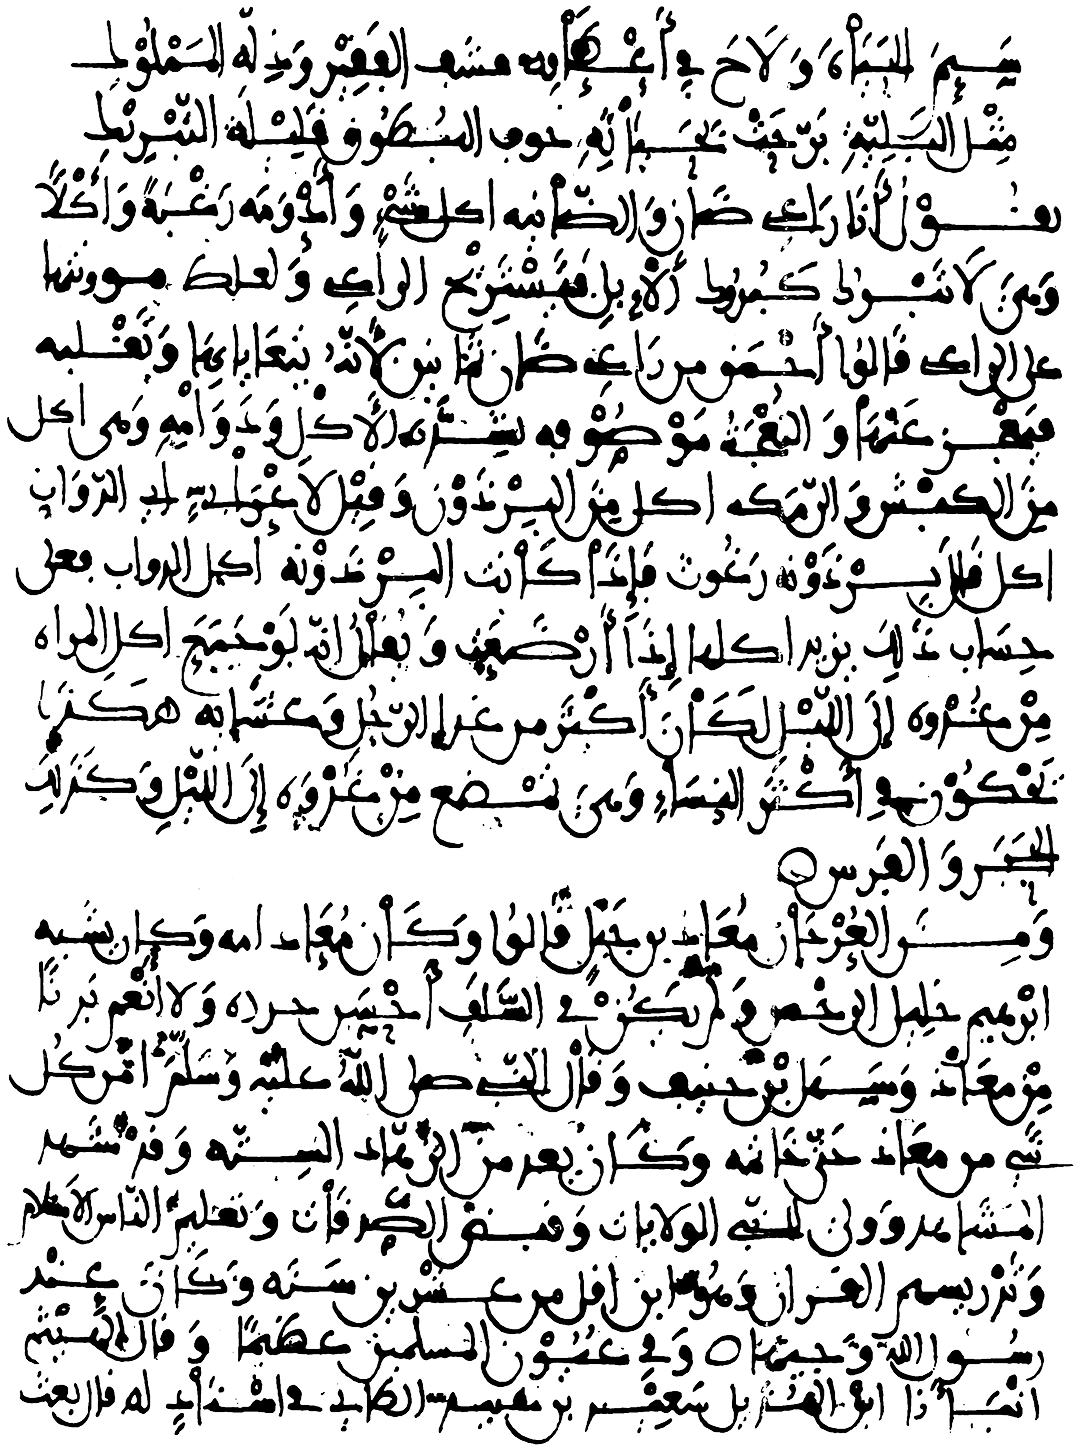
\includegraphics{img_116.png}
\caption[一个用阿拉伯语写成的有意义的故事。]
  {一个用阿拉伯语写成的有意义的故事。[摘自埃·卡蔷比与莫·西哲尔梅西[A. Khatibi; M. Sijelmassi],《伊斯兰书法大观》[\bn{The Splen-dour of Islamic Calligraphy}],纽约:Rizzoll, 1976年版。]}
\end{figure}

\section{关于思维的想象}

当然,我不能自欺欺人地以为在这些句子背后存在着意识——远非如此。在所有的人中,我最清楚为什么这个程序和真正的思维有着天壤之别。\emph{泰斯勒定理}在这里完全适用:一旦这个层次上的语言能力被机械化了,它就显然不再是智能的一部分了。但这种强烈的体验给我留下了一个想象:我隐隐约约地感到“真正的”思维是由大脑中更长、也更复杂的符号列车所组成的——许多列车同时沿许多彼此平行或交叉的轨道行驶,它们的车厢被推过去或拉过来,被挂上去或摘下来,被无数个神经转轨器从一条轨道上变换到另一条轨道上……

这是一个不可捉摸的想象,我无法用语言来表达它。它仅仅是个想象而已。但想象、直觉和动机在头脑中是紧密地混在一起的,而我对这个想象的极大兴趣不断地鞭策我更加深入地去思考思维到底是什么。我已经设法在本书的其它部分表达了一些从这个原始想象中派生出来的子想象——尤其是在《前奏曲,蚂蚁赋格》之中。

当我以十几年后的观点回顾这个程序的时候,现在我脑海里最强烈的感想是:在它所说的话背后缺乏形象感。这个程序不知道什么是农奴、什么是人,或任何其它事物。这些词只是空洞的形式符号,就像"pq"系统中的"p"和"q"那样空洞——或许比它们还要空洞。我的程序的优势来自这样一个事实:当人们读一段文字的时候,他们很自然地趋向于为每个词填满其全部意思——就像这些意思必然地附在形成该词的这些笔划上一样。我的程序可以被看作一个形式系统,它的“定理”——即输出的句子——具有既定的解释(至少对使用这种语言的人来说是这样)。但和"pq"系统不同,在这样解释了之后,这些“定理”并非都是真陈述。其中有许多是假的,还有许多是无意义的。

"pq"系统以其微不足道的方式反映了世界的一个小角落。但当我的程序运行时,在它的内部并未反映世界是如何运行的,它只反映了它所必须遵循的那一小组语义限制。为了能反映对世界的理解,我必须得为每个概念包裹上一层又一层关于世界的知识。这样做将是和我以前的做法不同的另一种努力。我并非没想过设法做到这一点——但我一直不知该怎么干。

\section{高层语法……}

事实上,我常常在思考我是否能写一个ATN语法(或某种其它的句子生成程序),它能只产生关于世界的“真”词句。这样一种语法能为每个词赋予名副其实的意义,就像在"pq"系统和TNT中所发生的那样。设计一种语言,使假陈述成为不合语法的,这个想法古已有之。这可以上溯到1633年的约翰·艾莫斯·夸美纽斯。这个想法很有吸引力,因为这样一来在你的语法中就嵌入了一块试金石:只需把你想要知道的陈述写下来,然后检查它是否合乎语法……实际上夸美纽斯走得更远,因为在他的语言里,假陈述不仅是不合语法的——它们根本就不可表示!

把这一思想引向另一个方向,你可以设想一个能生成随机公案的高层语法。为什么不可能呢?这种语法将等价于一个形式系统,其中的定理就是公案。而如果你有这样一个程序,你难道不能设法只生成“正宗的”公案吗?我的朋友玛莎·梅瑞狄丝热衷于这个“人工主义”的想法,因此她就着手编制一个公案书写程序。通过开始一段时间的努力,生成了下面这个古怪的“准公案”:

\begin{quote}
一个小的年轻禅师想要一个小的白色异形钵。“我们怎样才能不经过学习就能知道和理解呢?”这个年轻禅师问一个大的困惑着的禅师。这个困惑着的禅师带着一个小的红色的石钵从一座褐色的硬山走向一座白色的软山。这个困惑着的禅师看到了一个红色的软棚屋。这个困惑着的禅师想要这个棚屋。“菩提达摩为何要来中国?”这个困惑着的禅师问一个大的顿悟了的弟子。“桃子是大的”,这个弟子回答这个困惑着的禅师。“我们怎样才能不经过学习就能知道和理解呢?”这个困惑着的禅师问一个大的年老的禅师。这个年老的禅师来自一个白色的石G0025。这个年老的禅师消失了。
\end{quote}

你个人的关于公案正宗性的判定过程可能已经对此做出了判决,而不需要所谓“几何编码”或“禅宗串技艺”。如果代词的缺乏、句法的单一和语言的“现代化”还没有引起你的怀疑的话,临近结尾处那个奇怪的“G0025”也一定使你起了疑心。它是什么东西?它是一个奇怪的毛病——是一个故障的外部表现,这个故障使得原来应当打印出一个代表对象的词的地方被打印成了这个“节点”(事实上是Lisp中的一个原子)在程序中的内部名称,在这个节点中存储着关于这个特定对象的全部信息。因此我们在这里就有了一个“窗户”,透过它可以看到禅宗思想的低层——这一层本来是应当看不见的。不幸的是,我们无法在人的禅宗思想上开出来这样一个明晰地通向低层的窗户。

上面公案中的那一串行为的序列,尽管带有一些任意性,还是来自一个叫做“多级瀑布”的递归Lisp过程,这个过程构造出一个彼此通过不明确的因果方式相互联结的行动链。尽管这个公案生成程序对世界的理解程度显然没有高得令人惊讶,这项工作在使其输出看起来更加纯正这一点上还是取得了进步。

\section{音乐的语法?}

下一个问题是音乐。你开始可能会猜想这个领域很适合于被整理在一个ATN语法或其它类似的程序中。因为(把这个朴素的想法继续推进)语言必须从与外部世界的联系中获得意义,而音乐却纯粹是形式的。在乐曲的音响中不存在与“外在的”东西的关联,只存在纯粹的句法——一个音符接着一个音符、一个和弦接着一个和弦、一个小节接着一个小节、一个乐句接着一个乐句……

但请等等。在这段分析中有什么地方不大对头。为什么某些音乐要比其它音乐更深刻、更优美呢?这是因为音乐中的形式是具有表达力的——可以表达给我们头脑中某些奇特的潜意识区域。乐曲中的音响并不涉及农奴或者城邦,但它们触发了我们心灵最深处的模糊情感,在这个意义下,音乐的意义的确依赖于从符号到世界中的事物间的那些错综复杂的联系——在这种情况下,那些事物就是我们心中秘密的软件结构。不,伟大的音乐将不会出于像ATN语法这样简单的形式系统。伪音乐,像伪神话一样,是可能被产生出来的——对人来说这样做将是个有价值的尝试——但音乐中意义的秘密远不是靠纯粹的句法所能挖掘到的。

我在这里要明确一点:原则上说,ATN语法拥有任何程序化形式系统所具有的全部能力,因此如果音乐的意义归根结底是能以某种方式来加以把握的(我相信是这样的),那么一定能在一个ATN语法中被把握。这是真的。但在那种情况下,我仍然认为,这个语法的定义将不仅包含音乐结构,而且包含一个观察者的整个心智结构。这个语法将是全部思维的语法——而不仅仅是音乐的语法。

\section{维诺格拉德的程序“施徳鲁”}

哪种程序会被人承认为——即使是勉强地——具有一定的“理解力”?它要怎样做才能不使你直觉地感到其中“一无所有”?

在1968--1970年,特里·维诺格拉德(化名格拉德·维维诺诺博士)还是麻省理工学院的一个博士研究生,在研究同语言以及理解有关的课题。在当时的麻省理工学院,许多人工智能研究都涉及到所谓“积木世界”——一个相对简单的领域,很适于在其中处理涉及到视觉和计算机掌握语言的问题。积木世界中包括一张桌子,上面有各式各样的类似于儿童玩的那种积木——方的、长的、三角的、等等,各自有不同的颜色(作为另一种“积木世界”,请看\fig{117}:马格里特的画《心算》。我觉得这幅画的标题和内容再相配不过了)。在麻省理工学院的积木世界中,视觉问题是非常棘手的:一台计算机怎样才能通过对一个涉及到多块积木的场景进行电视扫描,指出其中有哪些种积木,以及它们之间的相互关系?某些积木可能叠在别的积木的上面,某些可能在另一些的前面,还有一些阴影,如此等等。

\begin{figure}
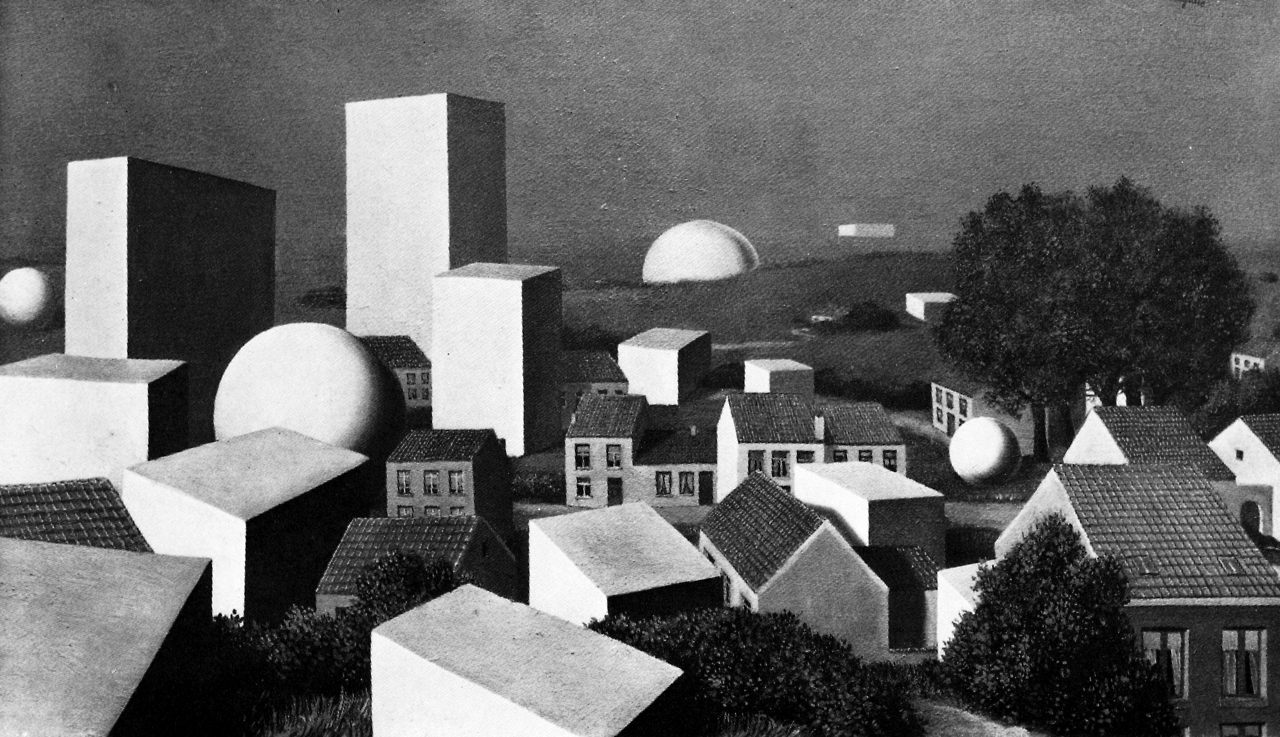
\includegraphics{img_117.jpg}
\caption[心算,马格里特作。]
  {心算,马格里特\pnum{1931}。}
\end{figure}

不过,维诺格拉德的工作是与视觉问题无关的。他开始时可以假设积木世界已经被良好地表示在计算机的存储器中了,而他所面临的任务是怎样让计算机完成下列工作:
\begin{enumerate}
\item 理解用自然语言表达的关于情境的问题;
\item 用自然语言回答关于情境的问题;
\item 理解用自然语言表达的处理积木的请求;
\item 把每个请求分解成由它所能执行的操作组成的序列;
\item 理解它所做的事情以及它这样做的原因;
\item 用自然语言叙述它的行动及其原因。
\end{enumerate}
一个貌似合理的想法是把整个程序分解成模块化的子程序,每个模块处理上述不同问题,然后,当这些模块都分别开发好了之后,再把它们适当地组合起来。但维诺格拉德发现,这种开发独立模块的策略会造成一些根本性的问题。他发展了一种激进的方法,向那些认为智能可以被划分成独立或半独立的部分的理论进行挑战。他的程序施德鲁并没有把问题分解成概念上清楚的若干组成部分。对句子做语法分析、生成内部表示、对其内部所表示的世界进行推理、回答问题等等,这一系列操作都以一种过程性的知识表示形式深深地、内在地纠缠在一起了。有些批评家曾指责他的程序过于错综复杂,以致于根本没有表示任何关于语言的“理论”,也没有以任何方式对我们理解思维过程有所贡献。在我看来这种主张简直是错得无以复加了。像施德鲁这样的杰作可能并不同构于我们的所做所为——事实上不管你采用什么方法,也无法认为施德鲁已经达到了“符号层”——但是在它的构造和分析过程中,却可以为我们认识智能的工作方式提供大量的材料。

\section{施德鲁的结构}

事实上,施德鲁不能分解成若干个独立的过程,其中每一个包含关于世界的某些知识。施德鲁中过程之间的相互依赖性很强,因此不能明确地相互分开。这个程序就像一个无法解开的复杂绳结,但你不能解开它这一事实并不意味着你不能理解它。即使这个绳结从物理上看错综复杂,对它仍可能有一个漂亮的几何描述。我们可以回到《一首无的奉献》中的那个比喻上去,把它比拟为从“自然的”角度观察一个果园。

维诺格拉德已经为施德鲁写下了清楚的说明。我要在这里引用他在一篇文章中的话,这篇文章收在尚克和科尔比所编的书中:

\begin{quote}
在这个模型中隐含的一个基本观点是:所有语言的使用都可以被看成是一种激活听话人心中的过程的手段。我们可以把任何言语表达都想象成一个程序——这个程序可以间接地导致一组操作,后者在听话人的认知系统中被执行。这种“程序的编写”是间接的,这就是说我们是在和一个有智能的解释者打交道,他有可能采用一组和说话人的意图极其不同的行为。这些行为的准确形式取决于他关于世界的知识,以及他对于与他谈话的人的预期,等等。在本程序中,我们为这个发生在机器人心中的解释过程提供了一个简单的形式。机器人所解释的每句话都被转换成一组用Planner语言表示的指令。然后再执行这样构造出来的程序,以达到预想的效果。\note{特里·维诺格拉德,“语言理解的过程性模型”,载于尚克和科尔比编的《思维与语言的计算机模型》,第170页。}
\end{quote}

\section{Planner为问题分解提供了方便}

这里提到的Planner语言是一种人工智能语言,它的基本特点是在其中设置了一些问题分解所需要的操作——比如说构造一棵包含子目标、子子目标等等的树的递归过程。这就是说,程序员不必每次不厌其烦地说明这棵树,它可以通过所谓“\inst{GOA}L[目标]语句”自动地被建立起来。读Planner程序的人不会看到这样的操作被明确地提到,用行话来说,他们是“对用户透明的”。如果树中的一条路径没能导致想要达到的目标,那么这个Planner程序将“回溯”并尝试另一个途径。只要提到Planner,就必须涉及“回溯”这个咒语。

维诺格拉德的程序出色地利用了Planner的这些特点——更准确地说,他用的是Microplanner-Planner方案的一个部分实现。但是,在过去的几年中,以发展人工智能为己任的人们已经认识到,Planner中所用的那种自动回溯具有无法避免的缺点,可能无法引导他们到达预想的目标。因此他们就从这条道上退了回来,想去试试完成人工智能的其它途径了。

让我们再听一些维诺格拉德关于施德鲁的解释:

\begin{quote}
每个词的定义都是一个程序,它将在分析过程中的适当时刻被调用,而且能对所涉及的句子和当前的外界情境进行任意运算。\note{维诺格拉德书,第175页。}
\end{quote}

维诺格拉德所举的例子中有下面这个:

\begin{quote}
“那个”\lnote{(英语的‘the’)}的不同可能意义对应于不同的过程,它们对上下文中的各种事实进行检查,然后规定一些行动,例如“在数据库中唯一地确定满足下列描述的对象”,或“断定所描述的对象在说话者看来肯定是唯一的”。在程序中包括了许多启发规则,它们被用来确定上下文中的哪些部分是有关的。\note{维诺格拉德书,第175页。}
\end{quote}

这个与“那个”这个词有关的问题的复杂程度是惊人的。保险的说法可能是:要想写一个程序来掌握最常用的五个词——汉语中是“的”、“了”、“是”、“一”、“不”;英语中是“the”、“of”、“and”、“a”、“to”——将等价于解决整个人工智能问题,因而也就相当于懂得了智能和意识到底是什么。稍微扯远一点,在汉语中五个最常用的名词——根据北京语言学院语言教学研究所编的《现代汉语频率词典》——是“上”、“人”、“里”、“年”、“天”(就是以这个次序)。关于这一点,令人惊奇的是大多数人想不到他们是这样用词的。如果你问问你的朋友,他们没准会猜想是“东西”、“问题”、“事情”、“同志”、“国家”这些词。另外,既然我们在考虑频率,非常值得一提的是在英语中最常用的$12$个字母——根据默根泰拉尔的统计——依次是“ETAOINSHRDLU”(这就是“伊她·娥英—施德鲁”的来历)。

施德鲁的一个有趣性质正好打击了那种认为计算机只善于处理数字的成见,这就是维诺格拉德所指出的一个事实:\quotetext{“我们的系统不是以数字的形式接受数目的,而且只被教会了数到十。”}\note{特里·维诺格拉德,《理解自然语言》,第69页。}尽管施德鲁是以数学为基础的,但它本身对数学却一窍不通!像马姨一样,施德鲁对于支撑着它的低级层次一无所知。它的知识在很大程度上是过程型的(参见前面对话的第11节中“格拉德·维维诺诺博士”的解释)。

如果把以过程的方式嵌入在施德鲁中的知识和我那个句子生成程序中的知识作一个对比,那将是很有趣的。我那个程序中全部句法知识都以过程的形式嵌入在扩充迁移网中,由Algol语言书写,但语义知识——关于语义类属关系的信息——却是静态的:它被装在每个词后面的一个短数字表中。有那么一些词,例如动词“是”、“有”等等,是完全表示在Algol过程中的,但它们是例外。与此相反,在施德鲁中所有的词都被表示成程序。这种情况说明,尽管数据和程序在理论上是等价的,在实际应用中选这个不选那个仍会造成很大的差别。

\section{句法和语义}

这里再引一段维诺格拉德的话:

\begin{quote}
我们的程序在运行时不是先对一个句子做句法分析,然后再做语义分析,最后使用演绎推理生成答案。在理解一句话的过程中,这三个活动始终是同时进行的。当一段句法结构开始形成的时候,一个语义程序被调用,以检查这个结构是否有意义,而由此产生的答案可以为句法分析提供指导。在确定它是否有意义的过程中,这个语义子程序可以调用演绎过程,并提出一些关于现实世界的问题。以对话中的第34句为例(“把蓝方锥搁在盒子里的蓝方块上头有问题吗?”),语法分析器先是认为“把蓝方锥搁在盒子里”是一个动词短语,这时语义分析就开始了,即检查在数据库中是否提到过下面这个事件:蓝方块把蓝方锥搁在盒子里。由于找不到这种事件,语法分析器又把“把蓝方锥搁在盒子里的蓝方块上头”理解为一个动词短语,即“问能不能做这样的事情”……这样在不同类的分析之间就有着不间断的相互作用,即一个的结果会对另一个发生影响。\note{维诺格拉德,“过程性模型”,第182--183页。译文有修改,以保持与对话一致。}
\end{quote}

在自然语言中句法和语义如此紧密地纠缠在一起,这是十分有趣的。在前一章关于“形式”这个难以捉摸的概念的讨论之中,我们已经把这个概念分成了两个范畴:句法形式——这是可以用一个预知可终止的判定过程来检查的——和语义形式——这是无法做上述检查的。但在这里,维诺格拉德告诫我们——至少在使用“句法”和“语义”的通常意义时是如此——它们在自然语言中是彼此混在一起的。一个句子的外部形式,即它由基本符号所组成的结构,是无法清楚地划分成句法和语义两部分的。这对语言学来说是极其重要的一点。

下面是维诺格拉德对施德鲁所作的一些最后的说明:

\begin{quote}
让我们看一下该系统对“一个支撑着方锥的红立方体”这样一个简单的描述是怎样处理的。这个描述将使用下列概念:“方块”、“红的”、“方锥”和“等边的”——它们都是系统中所含有的关于世界的范畴。其结果可以被表示成像\fig{118}所示的那种流程图。注意这是一个程序,它要寻找满足该描述的对象。然后可以把这个程序结合在一个命令中,这个命令可以对这个对象进行某种处理,对它提出某个问题,或者,如果它出现在一个语句中,它将成为程序的一部分,该程序的生成是为了表示特定的意义,以备后来使用。注意,在事先说明了第一条指令——找到方块X1——只查找一个特定对象的情况下,这段程序也可被用来检查该对象是否满足这一描述。

\begin{lrbox}{\TEMPBOX}%
\begin{tikzpicture}[trim right=(R),
  every node/.style={font=\normalfont\small}]
\path[node distance=5mm and 10mm,nodes=draw,
      JX/.style={inner sep=3mm},
      YX/.style={circle,inner sep=1mm},
      LX/.style={shape=diamond,shape aspect=3,inner xsep=0mm,inner ysep=.5mm}]
  node[name=A,YX]            {开始}
  node[name=B,JX,below=of A] {找到方块$\mathrm{X}1$}
  node[name=C,LX,below=of B] {$\mathrm{X}1$是红的吗?}
  node[name=D,LX,below=of C] {$\mathrm{X}1$是等边的吗?}
  node[name=E,JX,below=of D] {找到方锥$\mathrm{X}2$}
  node[name=F,LX,below=of E] {$\mathrm{X}1$是支撑着$\mathrm{X}2$吗?}
  node[name=G,YX,below=of F] {成功}
  node[name=H,YX,right=of {B-|current bounding box.east}] {失败};
\path[auto=left,->]
    (A) edge (B)
    (B) edge (C)
    (E) edge (F)
    (C) edge node{是} (D)
    (D) edge node{是} (E)
    (F) edge node{是} (G);
\draw[->] (F.west) -- ++(-5mm,0) coordinate (O) node[midway,above]{否} |- (E);
\draw[->] (D.west) -- (O |- D.west) node[midway,above]{否}
  |- ([yshift=2mm]B.west);
\draw[->] (C.west) -- ([xshift=4mm]O |- C.west) node[midway,above]{否}
  |- ([yshift=-2mm]B.west);
\draw[->] (E.east) -- (E.east -| {$(F.east)+(5mm,0)$}) coordinate (R)
  node[midway,above]{不再有} |- ($(B.east)-(0,2mm)$);
\draw[->] ([yshift=2mm]B.east) -- ([yshift=2mm]H.west)
  node[midway,above]{不再有};
\end{tikzpicture}
\end{lrbox}

\begin{figure}
%\includegraphics{img_118.png}
\fcapside[\FBwidth]{\usebox\TEMPBOX}{%
\caption[对“一个支撑着棱锥的红立方体”的过程化表示。]
  {对“一个支撑着方锥的红立方体”的过程化表示。[引自罗杰·尚克和肯尼恩·科尔比,《思维的计算机模型和语言》,172页。]}}
\end{figure}

这个程序刚一看上去似乎结构太复杂,因为我们不喜欢把一个简单语句想象成明显地含有循环、条件测试和其它的程序细节。解决的办法是提供一种内部语言,在其基本语句中包括适当的循环和测试,用这种语言来表示这一过程,就像前面那个描述一样简单了。\fig{118}所描述的程序可以被写成类似于下面所示的Planner程序:

\begin{tabbing}
\qquad\= \tabindent{-2em}\= \+\kill
$\mathrm{(GOAL(IS\ ?X1\ BLOCK))}$           \> 目标:$?\mathrm{X}1$是方形的 \\
$\mathrm{(GOAL(COLOR\text{-}OF\ ?X1\ RED))}$\> 目标:$?\mathrm{X}1$是红色的 \\
$\mathrm{(GOAL(EQUIDIMENSIONAL\ ?X1))}$     \> 目标:$?\mathrm{X}1$是等边的 \\
$\mathrm{(GOAL(IS\ ?X2\ PYRAMID))}$         \> 目标:$?\mathrm{X}2$是方锥体 \\
$\mathrm{(GOAL(SUPPORT\ ?X1\ ?X2))}$        \> 目标:$?\mathrm{X}1$支撑着$?\mathrm{X}2$
\end{tabbing}

流程图中的循环已隐含在Planner的回溯控制结构之中。这个描述的评价过程就是沿上述序列向下推进,直到某个目标失败为止,这时系统自动退回到前一个作出决定的地点,去尝试另一种可能性。一旦一个新对象名或“变量”\lnote{(变量名前面都有个“$?$”)}——如“$?\mathrm{X}1$”或“$?\mathrm{X}2$”——出现,就可作出一个决定。变量是由模式匹配程序来使用的。如果它们已经被指定代表某个特定的项,程序将检查对这个项来说该目标是否成立。如不成立,它将检查所有可能满足该目标的项,检查的方法是先挑选一个,然后一旦在这个地方出现了回溯,再去选下一个。这样,甚至检测和选择之间的区别都变成隐含的了。\note{维诺格拉德书,第171--172页。}
\end{quote}

在这个程序的设计过程中,一个重大的战略决策是不把自然语言全部翻译成Lisp语言,而是只翻译一半——翻译成Planner语言。这样(因为Planner解释程序本身是用Lisp写的),一个新的中间层——Planner——就被插入在顶层语言(自然语言)和底层语言(机器语言)之间了。这样,根据自然语言生成了Planner程序并将其送到Planner解释程序之后,施德鲁的高层就可以被解放出来,去处理新的任务了。

这种决定会不断地涌现:一个系统应当有多少层?在哪一层上该设置哪种“智能”?设置多少?这几个是人工智能在今天所面临的最困难的问题中的一部分。由于我们对自然智能所知甚少,所以很难说清人工智能系统的哪一层应该完成一个任务的哪一部分。

希望以上内容能帮助你管窥一下本章前面的对话场景背后的东西。在下一章中,我们将看到人工智能中一些新鲜的、推测性的想法。
